\documentclass[a4paper]{book}
\usepackage{makeidx}
\usepackage{graphicx}
\usepackage{multicol}
\usepackage{float}
\usepackage{listings}
\usepackage{color}
\usepackage{ifthen}
\usepackage[table]{xcolor}
\usepackage{textcomp}
\usepackage{alltt}
\usepackage{ifpdf}
\ifpdf
\usepackage[pdftex,
            pagebackref=true,
            colorlinks=true,
            linkcolor=blue,
            unicode
           ]{hyperref}
\else
\usepackage[ps2pdf,
            pagebackref=true,
            colorlinks=true,
            linkcolor=blue,
            unicode
           ]{hyperref}
\usepackage{pspicture}
\fi
\usepackage[utf8]{inputenc}
\usepackage{mathptmx}
\usepackage[scaled=.90]{helvet}
\usepackage{courier}
\usepackage{sectsty}
\usepackage[titles]{tocloft}
\usepackage{doxygen}
\lstset{language=C++,inputencoding=utf8,basicstyle=\footnotesize,breaklines=true,breakatwhitespace=true,tabsize=8,numbers=left }
\makeindex
\setcounter{tocdepth}{3}
\renewcommand{\footrulewidth}{0.4pt}
\renewcommand{\familydefault}{\sfdefault}
\begin{document}
\hypersetup{pageanchor=false}
\begin{titlepage}
\vspace*{7cm}
\begin{center}
{\Large Simulated Elevator \\[1ex]\large 0.1.0 }\\
\vspace*{1cm}
{\large Generated by Doxygen 1.7.4}\\
\vspace*{0.5cm}
{\small Mon Sep 5 2011 20:05:44}\\
\end{center}
\end{titlepage}
\clearemptydoublepage
\pagenumbering{roman}
\tableofcontents
\clearemptydoublepage
\pagenumbering{arabic}
\hypersetup{pageanchor=true}
\chapter{Class Index}
\section{Class List}
Here are the classes, structs, unions and interfaces with brief descriptions:\begin{DoxyCompactList}
\item\contentsline{section}{\hyperlink{class_dispatcher}{Dispatcher} }{\pageref{class_dispatcher}}{}
\item\contentsline{section}{\hyperlink{class_elevator}{Elevator} }{\pageref{class_elevator}}{}
\item\contentsline{section}{\hyperlink{class_main_window}{MainWindow} }{\pageref{class_main_window}}{}
\item\contentsline{section}{\hyperlink{class_receiver}{Receiver} }{\pageref{class_receiver}}{}
\item\contentsline{section}{\hyperlink{class_request}{Request} }{\pageref{class_request}}{}
\end{DoxyCompactList}

\chapter{Class Documentation}
\hypertarget{class_dispatcher}{
\section{Dispatcher Class Reference}
\label{class_dispatcher}\index{Dispatcher@{Dispatcher}}
}


{\ttfamily \#include $<$dispatcher.h$>$}

\subsection*{Public Slots}
\begin{DoxyCompactItemize}
\item 
void \hyperlink{class_dispatcher_a5fd444604d8eadaafac5791f9947f021}{requestReceived} (\hyperlink{class_request}{Request} $\ast$req)
\end{DoxyCompactItemize}
\subsection*{Public Member Functions}
\begin{DoxyCompactItemize}
\item 
\hyperlink{class_dispatcher_aa97cd04e05de526ce5d7f5bdba572f23}{Dispatcher} (QObject $\ast$parent=0)
\item 
void \hyperlink{class_dispatcher_a95437a6831a0f727a64d8490cf65a49f}{takeInControl} (\hyperlink{class_elevator}{Elevator} $\ast$elevator)
\end{DoxyCompactItemize}
\subsection*{Private Slots}
\begin{DoxyCompactItemize}
\item 
void \hyperlink{class_dispatcher_a5472cf1335843f5fa4655519b0e0bd94}{dispatchRequestPool} ()
\end{DoxyCompactItemize}
\subsection*{Private Attributes}
\begin{DoxyCompactItemize}
\item 
\hypertarget{class_dispatcher_ae261007a9a8d84ed18cd30c4694be2fa}{
QMap$<$ int, \hyperlink{class_elevator}{Elevator} $\ast$ $>$ \hyperlink{class_dispatcher_ae261007a9a8d84ed18cd30c4694be2fa}{elevators}}
\label{class_dispatcher_ae261007a9a8d84ed18cd30c4694be2fa}

\begin{DoxyCompactList}\small\item\em List of the elevators taken into control. \end{DoxyCompactList}\item 
\hypertarget{class_dispatcher_a93d6aeb2b2dcb6383f7f1522ac4695dd}{
QList$<$ \hyperlink{class_request}{Request} $\ast$ $>$ \hyperlink{class_dispatcher_a93d6aeb2b2dcb6383f7f1522ac4695dd}{requestPool}}
\label{class_dispatcher_a93d6aeb2b2dcb6383f7f1522ac4695dd}

\begin{DoxyCompactList}\small\item\em List of requests unable to dispatch (Waiting for dispatch) \end{DoxyCompactList}\end{DoxyCompactItemize}


\subsection{Detailed Description}
\hyperlink{class_dispatcher}{Dispatcher} Object Receive requests and decide which elevator should take the job 

\subsection{Constructor \& Destructor Documentation}
\hypertarget{class_dispatcher_aa97cd04e05de526ce5d7f5bdba572f23}{
\index{Dispatcher@{Dispatcher}!Dispatcher@{Dispatcher}}
\index{Dispatcher@{Dispatcher}!Dispatcher@{Dispatcher}}
\subsubsection[{Dispatcher}]{\setlength{\rightskip}{0pt plus 5cm}Dispatcher::Dispatcher (
\begin{DoxyParamCaption}
\item[{QObject $\ast$}]{parent = {\ttfamily 0}}
\end{DoxyParamCaption}
)\hspace{0.3cm}{\ttfamily  \mbox{[}inline, explicit\mbox{]}}}}
\label{class_dispatcher_aa97cd04e05de526ce5d7f5bdba572f23}
Construct a \hyperlink{class_dispatcher}{Dispatcher} object 

\subsection{Member Function Documentation}
\hypertarget{class_dispatcher_a5472cf1335843f5fa4655519b0e0bd94}{
\index{Dispatcher@{Dispatcher}!dispatchRequestPool@{dispatchRequestPool}}
\index{dispatchRequestPool@{dispatchRequestPool}!Dispatcher@{Dispatcher}}
\subsubsection[{dispatchRequestPool}]{\setlength{\rightskip}{0pt plus 5cm}void Dispatcher::dispatchRequestPool (
\begin{DoxyParamCaption}
{}
\end{DoxyParamCaption}
)\hspace{0.3cm}{\ttfamily  \mbox{[}inline, private, slot\mbox{]}}}}
\label{class_dispatcher_a5472cf1335843f5fa4655519b0e0bd94}
Slot invoked to try to dispatch the \hyperlink{class_request}{Request} in requestPool to the most suitable \hyperlink{class_elevator}{Elevator} 

Here is the call graph for this function:\nopagebreak
\begin{figure}[H]
\begin{center}
\leavevmode
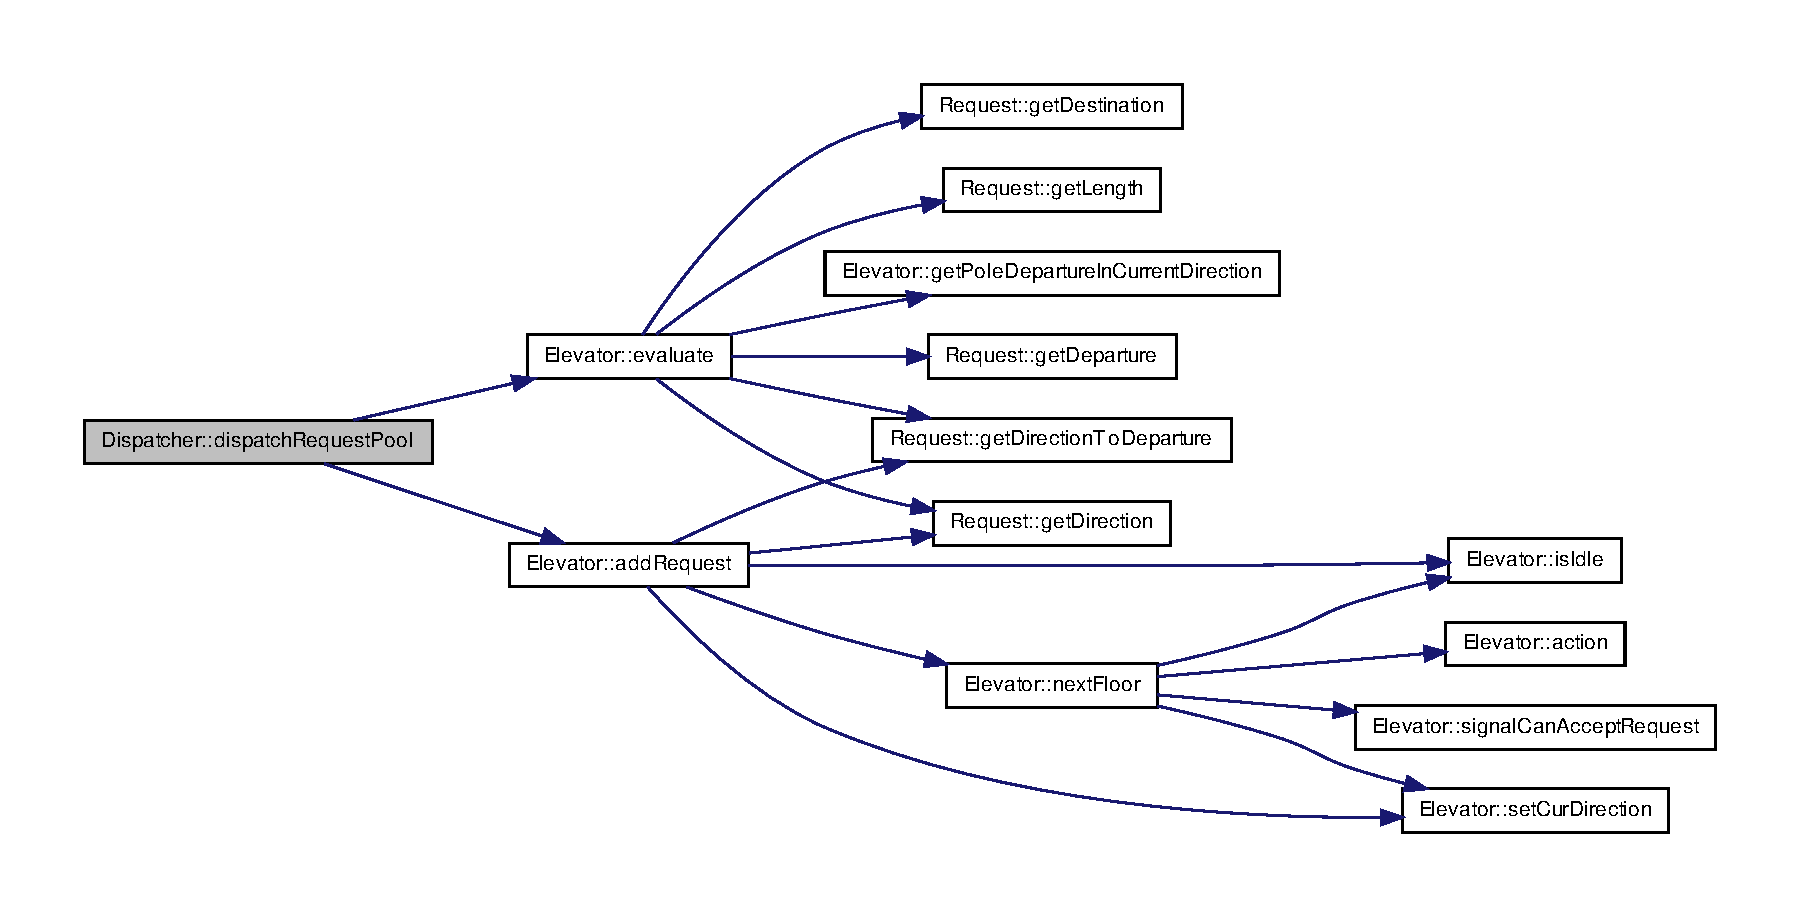
\includegraphics[width=400pt]{class_dispatcher_a5472cf1335843f5fa4655519b0e0bd94_cgraph}
\end{center}
\end{figure}




Here is the caller graph for this function:\nopagebreak
\begin{figure}[H]
\begin{center}
\leavevmode
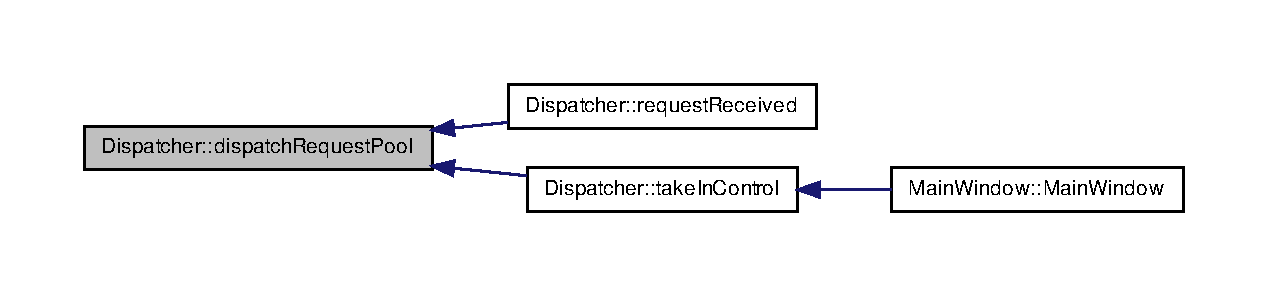
\includegraphics[width=400pt]{class_dispatcher_a5472cf1335843f5fa4655519b0e0bd94_icgraph}
\end{center}
\end{figure}


\hypertarget{class_dispatcher_a5fd444604d8eadaafac5791f9947f021}{
\index{Dispatcher@{Dispatcher}!requestReceived@{requestReceived}}
\index{requestReceived@{requestReceived}!Dispatcher@{Dispatcher}}
\subsubsection[{requestReceived}]{\setlength{\rightskip}{0pt plus 5cm}void Dispatcher::requestReceived (
\begin{DoxyParamCaption}
\item[{{\bf Request} $\ast$}]{req}
\end{DoxyParamCaption}
)\hspace{0.3cm}{\ttfamily  \mbox{[}inline, slot\mbox{]}}}}
\label{class_dispatcher_a5fd444604d8eadaafac5791f9947f021}
Slot for the dispatcher to obtain the \hyperlink{class_request}{Request} 

Here is the call graph for this function:\nopagebreak
\begin{figure}[H]
\begin{center}
\leavevmode
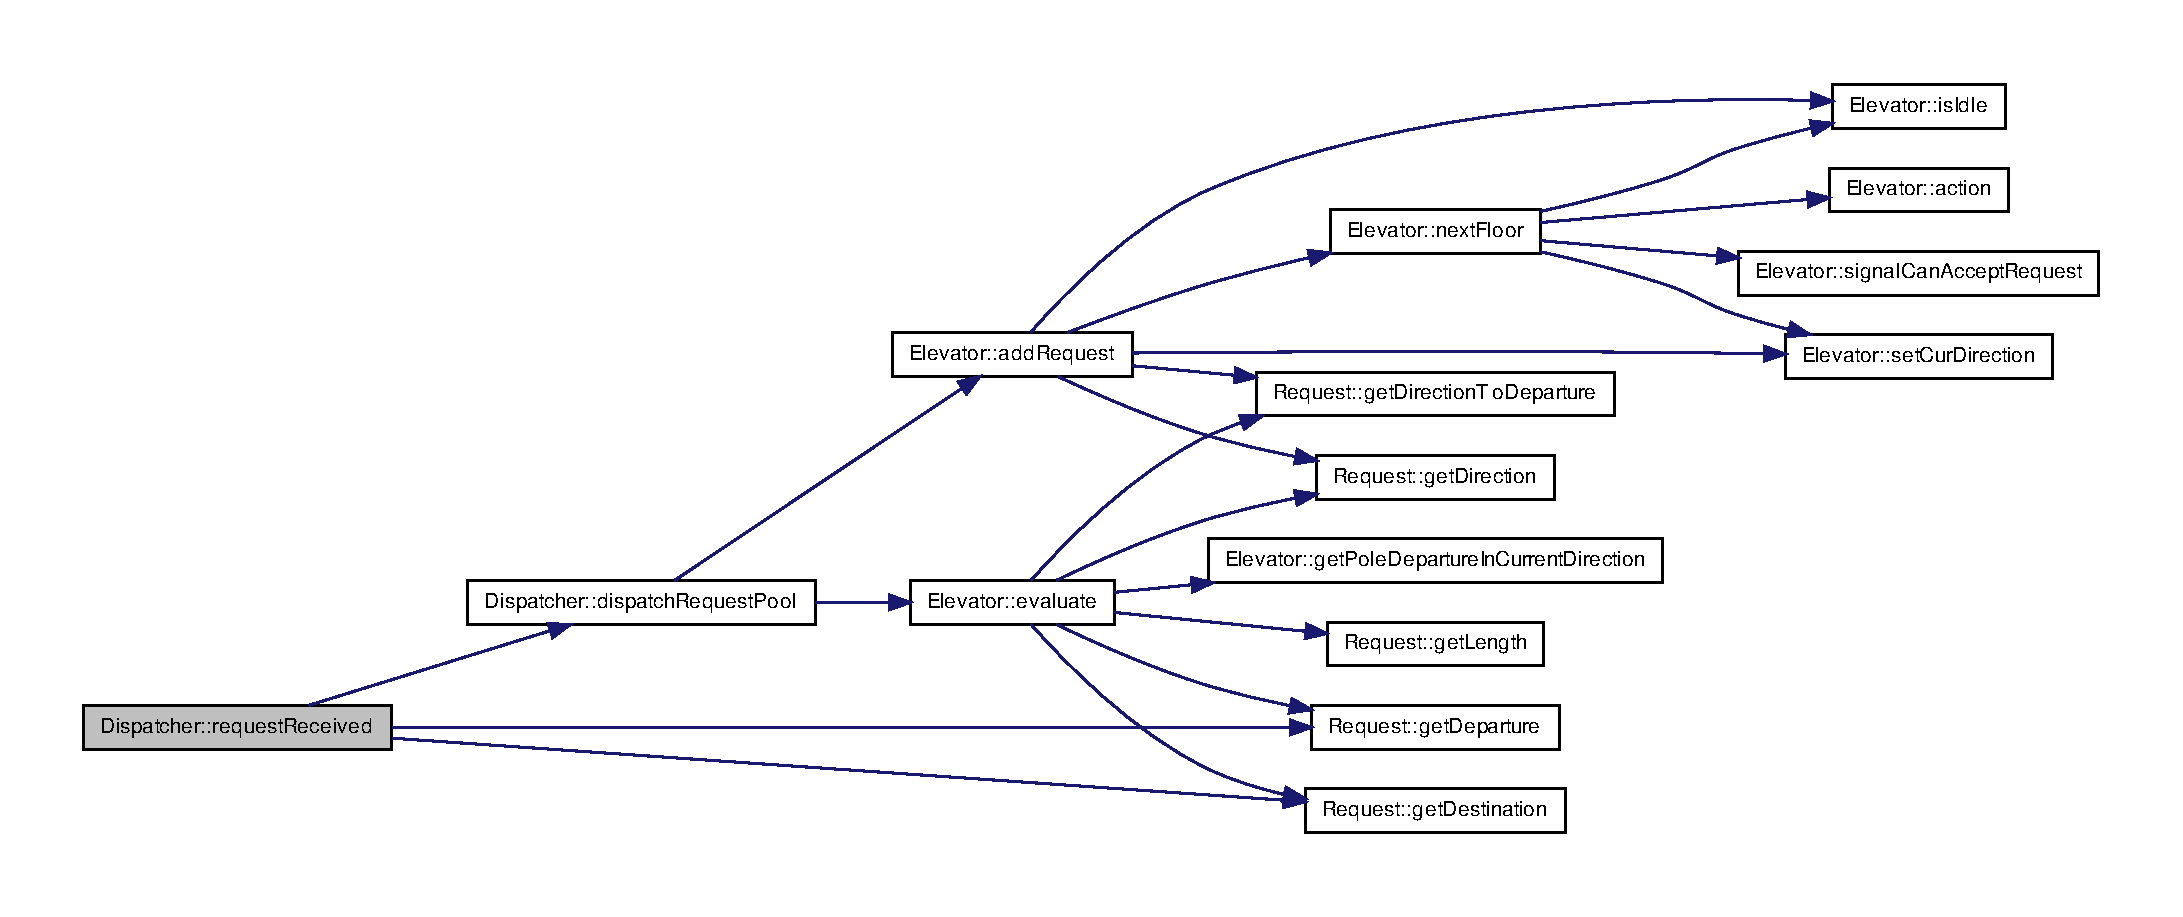
\includegraphics[width=400pt]{class_dispatcher_a5fd444604d8eadaafac5791f9947f021_cgraph}
\end{center}
\end{figure}


\hypertarget{class_dispatcher_a95437a6831a0f727a64d8490cf65a49f}{
\index{Dispatcher@{Dispatcher}!takeInControl@{takeInControl}}
\index{takeInControl@{takeInControl}!Dispatcher@{Dispatcher}}
\subsubsection[{takeInControl}]{\setlength{\rightskip}{0pt plus 5cm}void Dispatcher::takeInControl (
\begin{DoxyParamCaption}
\item[{{\bf Elevator} $\ast$}]{elevator}
\end{DoxyParamCaption}
)\hspace{0.3cm}{\ttfamily  \mbox{[}inline\mbox{]}}}}
\label{class_dispatcher_a95437a6831a0f727a64d8490cf65a49f}
Register an \hyperlink{class_elevator}{Elevator} object. So that when a request is received, the \hyperlink{class_elevator}{Elevator} will be taken in to consideration to dispatch the request. 

Here is the call graph for this function:\nopagebreak
\begin{figure}[H]
\begin{center}
\leavevmode
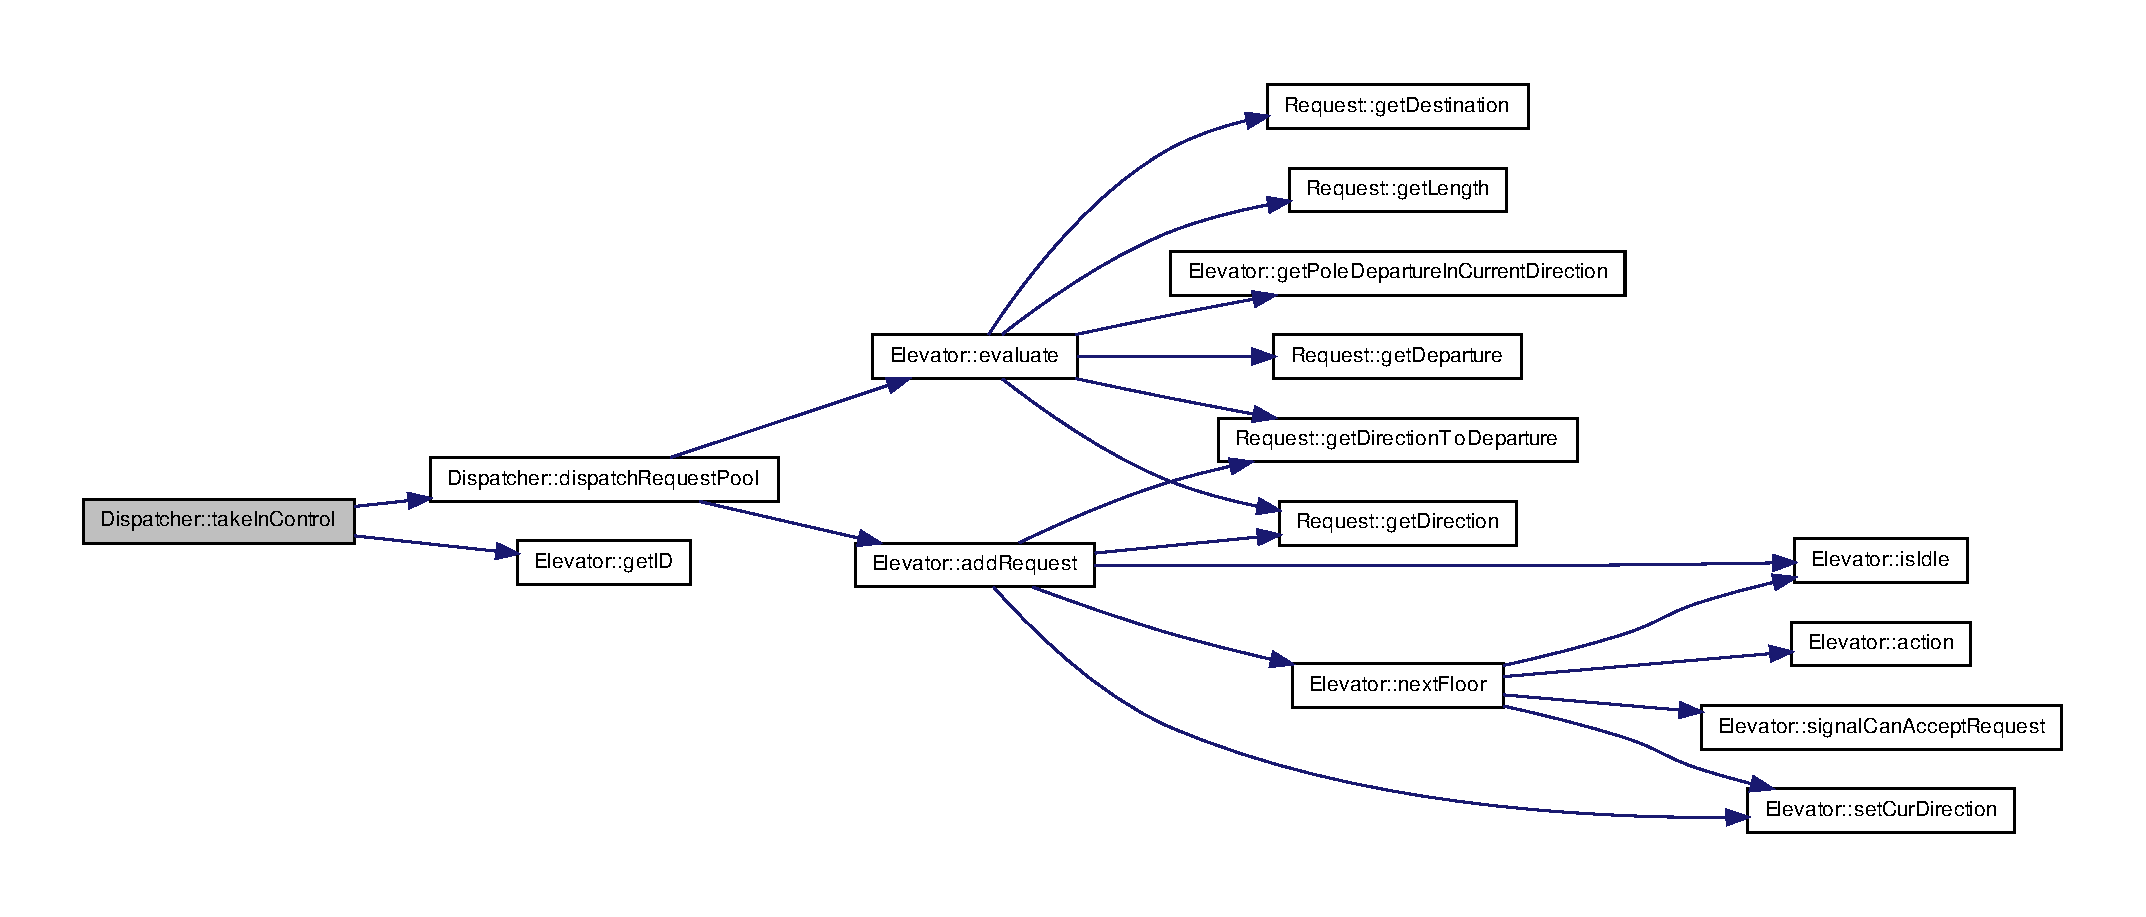
\includegraphics[width=400pt]{class_dispatcher_a95437a6831a0f727a64d8490cf65a49f_cgraph}
\end{center}
\end{figure}




Here is the caller graph for this function:\nopagebreak
\begin{figure}[H]
\begin{center}
\leavevmode
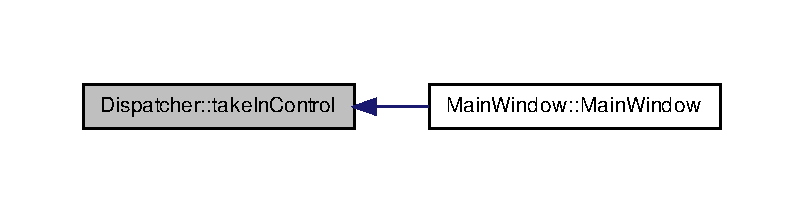
\includegraphics[width=386pt]{class_dispatcher_a95437a6831a0f727a64d8490cf65a49f_icgraph}
\end{center}
\end{figure}




The documentation for this class was generated from the following file:\begin{DoxyCompactItemize}
\item 
dispatcher.h\end{DoxyCompactItemize}

\hypertarget{class_elevator}{
\section{Elevator Class Reference}
\label{class_elevator}\index{Elevator@{Elevator}}
}


{\ttfamily \#include $<$elevator.h$>$}

\subsection*{Signals}
\begin{DoxyCompactItemize}
\item 
void \hyperlink{class_elevator_a688a7f343cc5d4ceec45feea140ccba2}{signalCanAcceptRequest} (int elevatorIndex)
\end{DoxyCompactItemize}
\subsection*{Public Member Functions}
\begin{DoxyCompactItemize}
\item 
\hyperlink{class_elevator_a1d3d0e6613a99a780dc2a14935ed47ec}{Elevator} (QWidget $\ast$parent=0, int index=-\/1)
\item 
int \hyperlink{class_elevator_aca5f48d0086a5791d6fa822c4efc4d96}{getID} ()
\item 
int \hyperlink{class_elevator_a2e9a499fe4d2b2ccff043d3798399743}{evaluate} (\hyperlink{class_request}{Request} $\ast$req)
\item 
bool \hyperlink{class_elevator_aaef88b9050a598bfc711e0f4a55711d0}{addRequest} (\hyperlink{class_request}{Request} $\ast$req)
\item 
int \hyperlink{class_elevator_a333ca5f86534823e1efda55e48c36abe}{getCurrentFloor} ()
\item 
bool \hyperlink{class_elevator_a64dc8a888c4ae8914a2ce640b3104c39}{isIdle} ()
\end{DoxyCompactItemize}
\subsection*{Static Public Attributes}
\begin{DoxyCompactItemize}
\item 
\hypertarget{class_elevator_a457c6551bbec5edc5051c381ed8cb037}{
static int \hyperlink{class_elevator_a457c6551bbec5edc5051c381ed8cb037}{indexSequence} = 0}
\label{class_elevator_a457c6551bbec5edc5051c381ed8cb037}

\begin{DoxyCompactList}\small\item\em Global \hyperlink{class_elevator}{Elevator} Count Variable (Used for generate default id) \end{DoxyCompactList}\item 
\hypertarget{class_elevator_a0e992da73960fcb066c4216d48828348}{
static const int \hyperlink{class_elevator_a0e992da73960fcb066c4216d48828348}{FLOOR\_\-NONE} = -\/1}
\label{class_elevator_a0e992da73960fcb066c4216d48828348}

\begin{DoxyCompactList}\small\item\em Value for a floor number hich means unavaliable. \end{DoxyCompactList}\item 
\hypertarget{class_elevator_aea037729441aae59042ce4f5b9b3adf7}{
static const int \hyperlink{class_elevator_aea037729441aae59042ce4f5b9b3adf7}{REQUEST\_\-UNACCEPTABLE} = -\/1}
\label{class_elevator_aea037729441aae59042ce4f5b9b3adf7}

\begin{DoxyCompactList}\small\item\em Cost for a request that can't be accept by this elevator anyway. \end{DoxyCompactList}\end{DoxyCompactItemize}
\subsection*{Private Slots}
\begin{DoxyCompactItemize}
\item 
void \hyperlink{class_elevator_a1c7640e845ad36870c764f87e53d21e2}{animeDoorOpenFinished} ()
\item 
void \hyperlink{class_elevator_ad0d2554d24ea14d07afa2a7e5d00725a}{animePassengersFinished} ()
\item 
void \hyperlink{class_elevator_a5d4ecef44a3e87b14b5ce8de10008fdd}{nextFloor} ()
\item 
int \hyperlink{class_elevator_abd54853d9aba7177792df167c0bb894c}{getPoleDepartureInCurrentDirection} ()
\end{DoxyCompactItemize}
\subsection*{Private Member Functions}
\begin{DoxyCompactItemize}
\item 
void \hyperlink{class_elevator_ac9f33c34d59902f14c72bc86c6c3edb7}{action} (\hyperlink{class_request_a31872cb7919df688dc6866ea607b9d9d}{Request::DIRECTION} \hyperlink{class_elevator_a0e5685fa3ebcfb3c5e4810adc6c5388a}{direction}=Request::DIRECTION\_\-NONE)
\item 
void \hyperlink{class_elevator_a92dbf1fd3ff98c4656ee428b43a35a4c}{createAnimations} ()
\item 
void \hyperlink{class_elevator_aabecded393aa00b30a1f2071b0ae1cdd}{createAnimationMove} ()
\item 
void \hyperlink{class_elevator_a49c56159bb74facd0661c40f621b886f}{createAnimationDoor} ()
\item 
void \hyperlink{class_elevator_ad854f6f6fa0d4c8b6066edc1282fced3}{setCurDirection} (\hyperlink{class_request_a31872cb7919df688dc6866ea607b9d9d}{Request::DIRECTION} curDir)
\end{DoxyCompactItemize}
\subsection*{Private Attributes}
\begin{DoxyCompactItemize}
\item 
\hypertarget{class_elevator_a008833dba4a008951035b3ab1ca9231a}{
Ui::Elevator $\ast$ \hyperlink{class_elevator_a008833dba4a008951035b3ab1ca9231a}{ui}}
\label{class_elevator_a008833dba4a008951035b3ab1ca9231a}

\begin{DoxyCompactList}\small\item\em Qt UI object of \hyperlink{class_elevator}{Elevator}. \end{DoxyCompactList}\item 
\hypertarget{class_elevator_aa31e06e205c1c29028deafa7ecff4ae8}{
int \hyperlink{class_elevator_aa31e06e205c1c29028deafa7ecff4ae8}{id}}
\label{class_elevator_aa31e06e205c1c29028deafa7ecff4ae8}

\begin{DoxyCompactList}\small\item\em ID(Index) of the current elevator. \end{DoxyCompactList}\item 
\hypertarget{class_elevator_a07597b24e92d6a74db2c97035edd225e}{
int \hyperlink{class_elevator_a07597b24e92d6a74db2c97035edd225e}{curFloor}}
\label{class_elevator_a07597b24e92d6a74db2c97035edd225e}

\begin{DoxyCompactList}\small\item\em Floornumber the \hyperlink{class_elevator}{Elevator} is now. \end{DoxyCompactList}\item 
\hypertarget{class_elevator_a29320516a530002a9156fcaf6b006a91}{
int \hyperlink{class_elevator_a29320516a530002a9156fcaf6b006a91}{inPassengerCount}}
\label{class_elevator_a29320516a530002a9156fcaf6b006a91}

\begin{DoxyCompactList}\small\item\em Number of people come into the \hyperlink{class_elevator}{Elevator} after door opened. \end{DoxyCompactList}\item 
\hypertarget{class_elevator_a2ddde08d62ca990aa07160e45f3eef0e}{
int \hyperlink{class_elevator_a2ddde08d62ca990aa07160e45f3eef0e}{outPassengerCount}}
\label{class_elevator_a2ddde08d62ca990aa07160e45f3eef0e}

\begin{DoxyCompactList}\small\item\em Number of people go outof the \hyperlink{class_elevator}{Elevator} after door opened. \end{DoxyCompactList}\item 
\hypertarget{class_elevator_ad650e2c1962ac39ee93b33b52d30c824}{
int \hyperlink{class_elevator_ad650e2c1962ac39ee93b33b52d30c824}{passengerCount}}
\label{class_elevator_ad650e2c1962ac39ee93b33b52d30c824}

\begin{DoxyCompactList}\small\item\em Number of people in the \hyperlink{class_elevator}{Elevator}. \end{DoxyCompactList}\item 
\hypertarget{class_elevator_a700abab6b67b912087607a94fa194110}{
\hyperlink{class_request_a31872cb7919df688dc6866ea607b9d9d}{Request::DIRECTION} \hyperlink{class_elevator_a700abab6b67b912087607a94fa194110}{curDirection}}
\label{class_elevator_a700abab6b67b912087607a94fa194110}

\begin{DoxyCompactList}\small\item\em Current running DIRECTION. \end{DoxyCompactList}\item 
\hypertarget{class_elevator_a0e5685fa3ebcfb3c5e4810adc6c5388a}{
\hyperlink{class_request_a31872cb7919df688dc6866ea607b9d9d}{Request::DIRECTION} \hyperlink{class_elevator_a0e5685fa3ebcfb3c5e4810adc6c5388a}{direction}}
\label{class_elevator_a0e5685fa3ebcfb3c5e4810adc6c5388a}

\begin{DoxyCompactList}\small\item\em DIRECTION of the first request. \end{DoxyCompactList}\item 
\hypertarget{class_elevator_ab64bb0f856260d8bac401c96618ccb36}{
QList$<$ \hyperlink{class_request}{Request} $\ast$ $>$ \hyperlink{class_elevator_ab64bb0f856260d8bac401c96618ccb36}{requests}}
\label{class_elevator_ab64bb0f856260d8bac401c96618ccb36}

\begin{DoxyCompactList}\small\item\em List of the tasks to do. \end{DoxyCompactList}\item 
\hypertarget{class_elevator_a5d2c79ac63afc0891c97ad4e65cac2a9}{
QSequentialAnimationGroup $\ast$ \hyperlink{class_elevator_a5d2c79ac63afc0891c97ad4e65cac2a9}{animeDoorOpen}}
\label{class_elevator_a5d2c79ac63afc0891c97ad4e65cac2a9}

\begin{DoxyCompactList}\small\item\em Animation object: Open the door of the \hyperlink{class_elevator}{Elevator}. \end{DoxyCompactList}\item 
\hypertarget{class_elevator_ac46d5a0a1fb9094138d771cfb1d5e632}{
QParallelAnimationGroup $\ast$ \hyperlink{class_elevator_ac46d5a0a1fb9094138d771cfb1d5e632}{animePassengers}}
\label{class_elevator_ac46d5a0a1fb9094138d771cfb1d5e632}

\begin{DoxyCompactList}\small\item\em Animation object: People come in and out of the \hyperlink{class_elevator}{Elevator}. \end{DoxyCompactList}\item 
\hypertarget{class_elevator_a34b7927963bedf4ba7727e83e53706cb}{
QSequentialAnimationGroup $\ast$ \hyperlink{class_elevator_a34b7927963bedf4ba7727e83e53706cb}{animeDoorClose}}
\label{class_elevator_a34b7927963bedf4ba7727e83e53706cb}

\begin{DoxyCompactList}\small\item\em Animation object: Close the door of the \hyperlink{class_elevator}{Elevator}. \end{DoxyCompactList}\item 
\hypertarget{class_elevator_a3fece615cc6c5f0123d4731021ae683a}{
QParallelAnimationGroup $\ast$ \hyperlink{class_elevator_a3fece615cc6c5f0123d4731021ae683a}{animeUpward}}
\label{class_elevator_a3fece615cc6c5f0123d4731021ae683a}

\begin{DoxyCompactList}\small\item\em Animation object: Move the \hyperlink{class_elevator}{Elevator} up. \end{DoxyCompactList}\item 
\hypertarget{class_elevator_af14b33b5234414d0c90a8328f9b0fffa}{
QParallelAnimationGroup $\ast$ \hyperlink{class_elevator_af14b33b5234414d0c90a8328f9b0fffa}{animeDownward}}
\label{class_elevator_af14b33b5234414d0c90a8328f9b0fffa}

\begin{DoxyCompactList}\small\item\em Animation object: Move the \hyperlink{class_elevator}{Elevator} down. \end{DoxyCompactList}\item 
\hypertarget{class_elevator_a1f9815d1977acf5312fe26a6311e0818}{
QParallelAnimationGroup $\ast$ \hyperlink{class_elevator_a1f9815d1977acf5312fe26a6311e0818}{animeGrpParallel}}
\label{class_elevator_a1f9815d1977acf5312fe26a6311e0818}

\begin{DoxyCompactList}\small\item\em Animation object: Temporary object. \end{DoxyCompactList}\item 
\hypertarget{class_elevator_a14ba7f0b2e17e3e1a6dcae034ba914e6}{
QSequentialAnimationGroup $\ast$ \hyperlink{class_elevator_a14ba7f0b2e17e3e1a6dcae034ba914e6}{animeGrpSequential}}
\label{class_elevator_a14ba7f0b2e17e3e1a6dcae034ba914e6}

\begin{DoxyCompactList}\small\item\em Animation object: Temporary object. \end{DoxyCompactList}\item 
\hypertarget{class_elevator_a32e33134fc75b79f3ca1a5fbe08b8e12}{
QPropertyAnimation $\ast$ \hyperlink{class_elevator_a32e33134fc75b79f3ca1a5fbe08b8e12}{anime}}
\label{class_elevator_a32e33134fc75b79f3ca1a5fbe08b8e12}

\begin{DoxyCompactList}\small\item\em Animation object: Temporary object. \end{DoxyCompactList}\end{DoxyCompactItemize}


\subsection{Detailed Description}
\hyperlink{class_elevator}{Elevator} Class Run according to a \hyperlink{class_request}{Request} List, Carry passengers and most important, play animation 

\subsection{Constructor \& Destructor Documentation}
\hypertarget{class_elevator_a1d3d0e6613a99a780dc2a14935ed47ec}{
\index{Elevator@{Elevator}!Elevator@{Elevator}}
\index{Elevator@{Elevator}!Elevator@{Elevator}}
\subsubsection[{Elevator}]{\setlength{\rightskip}{0pt plus 5cm}Elevator::Elevator (
\begin{DoxyParamCaption}
\item[{QWidget $\ast$}]{parent = {\ttfamily 0}, }
\item[{int}]{index = {\ttfamily -\/1}}
\end{DoxyParamCaption}
)\hspace{0.3cm}{\ttfamily  \mbox{[}inline, explicit\mbox{]}}}}
\label{class_elevator_a1d3d0e6613a99a780dc2a14935ed47ec}
Construct an \hyperlink{class_elevator}{Elevator}. If the index in param list not specificed sequential value will be used. 

Here is the call graph for this function:\nopagebreak
\begin{figure}[H]
\begin{center}
\leavevmode
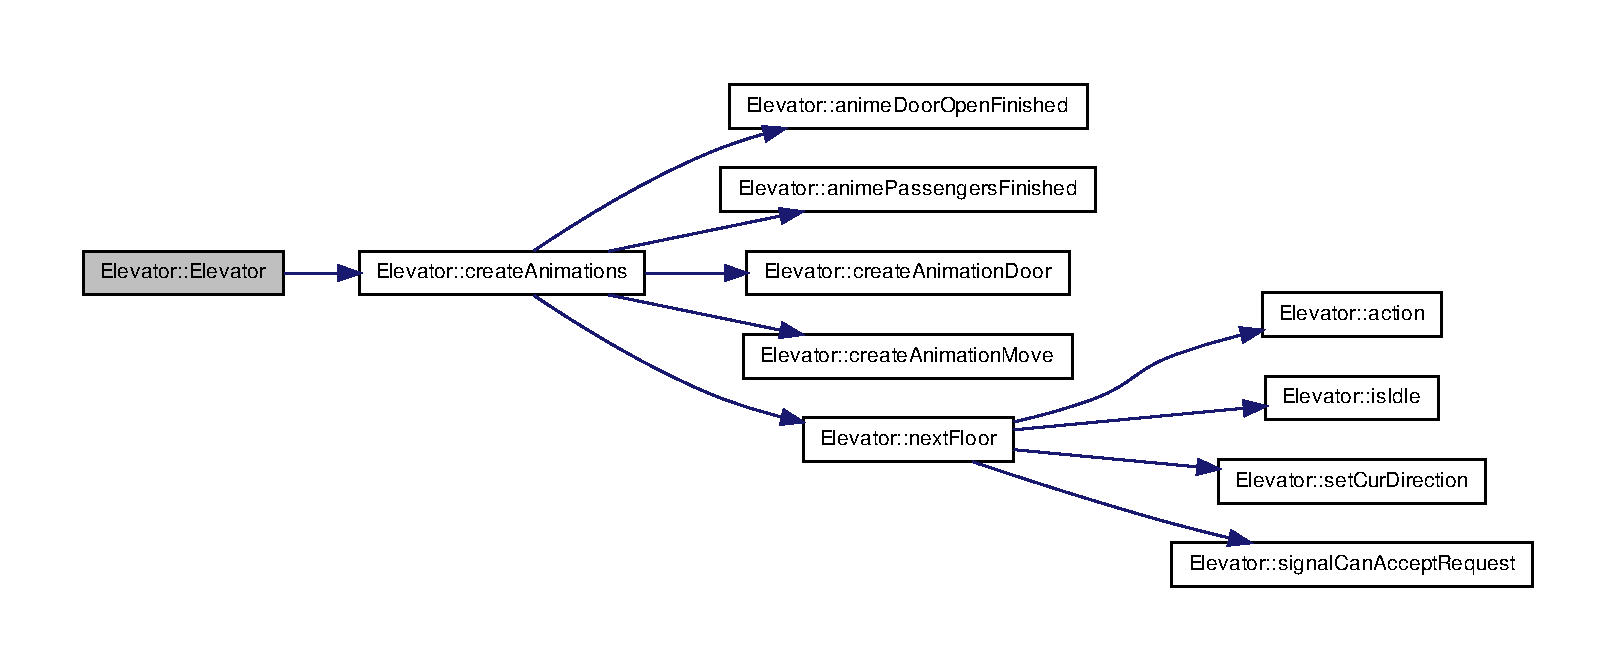
\includegraphics[width=400pt]{class_elevator_a1d3d0e6613a99a780dc2a14935ed47ec_cgraph}
\end{center}
\end{figure}




\subsection{Member Function Documentation}
\hypertarget{class_elevator_ac9f33c34d59902f14c72bc86c6c3edb7}{
\index{Elevator@{Elevator}!action@{action}}
\index{action@{action}!Elevator@{Elevator}}
\subsubsection[{action}]{\setlength{\rightskip}{0pt plus 5cm}void Elevator::action (
\begin{DoxyParamCaption}
\item[{{\bf Request::DIRECTION}}]{direction = {\ttfamily Request::DIRECTION\_\-NONE}}
\end{DoxyParamCaption}
)\hspace{0.3cm}{\ttfamily  \mbox{[}inline, private\mbox{]}}}}
\label{class_elevator_ac9f33c34d59902f14c72bc86c6c3edb7}
Play animations with this function 

Here is the caller graph for this function:\nopagebreak
\begin{figure}[H]
\begin{center}
\leavevmode
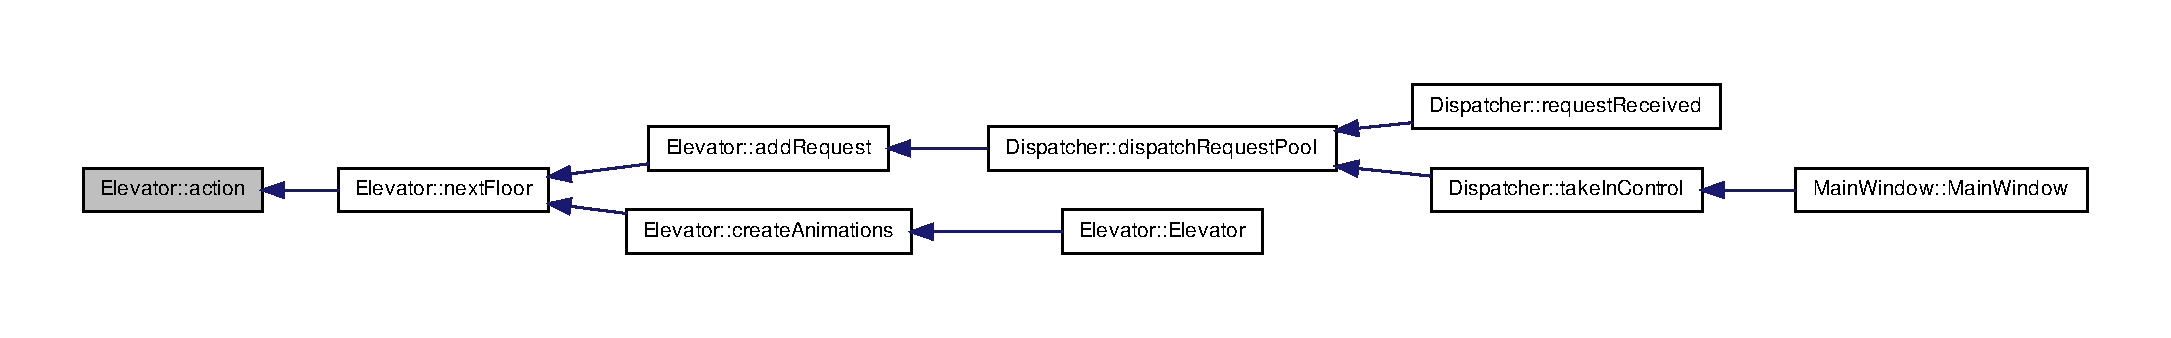
\includegraphics[width=400pt]{class_elevator_ac9f33c34d59902f14c72bc86c6c3edb7_icgraph}
\end{center}
\end{figure}


\hypertarget{class_elevator_aaef88b9050a598bfc711e0f4a55711d0}{
\index{Elevator@{Elevator}!addRequest@{addRequest}}
\index{addRequest@{addRequest}!Elevator@{Elevator}}
\subsubsection[{addRequest}]{\setlength{\rightskip}{0pt plus 5cm}bool Elevator::addRequest (
\begin{DoxyParamCaption}
\item[{{\bf Request} $\ast$}]{req}
\end{DoxyParamCaption}
)\hspace{0.3cm}{\ttfamily  \mbox{[}inline\mbox{]}}}}
\label{class_elevator_aaef88b9050a598bfc711e0f4a55711d0}
Insert a request to the working list of the \hyperlink{class_elevator}{Elevator}. \par
 Out of the trust to \hyperlink{class_dispatcher}{Dispatcher}, addRequest will not check the avaliability of a request! 

Here is the call graph for this function:\nopagebreak
\begin{figure}[H]
\begin{center}
\leavevmode
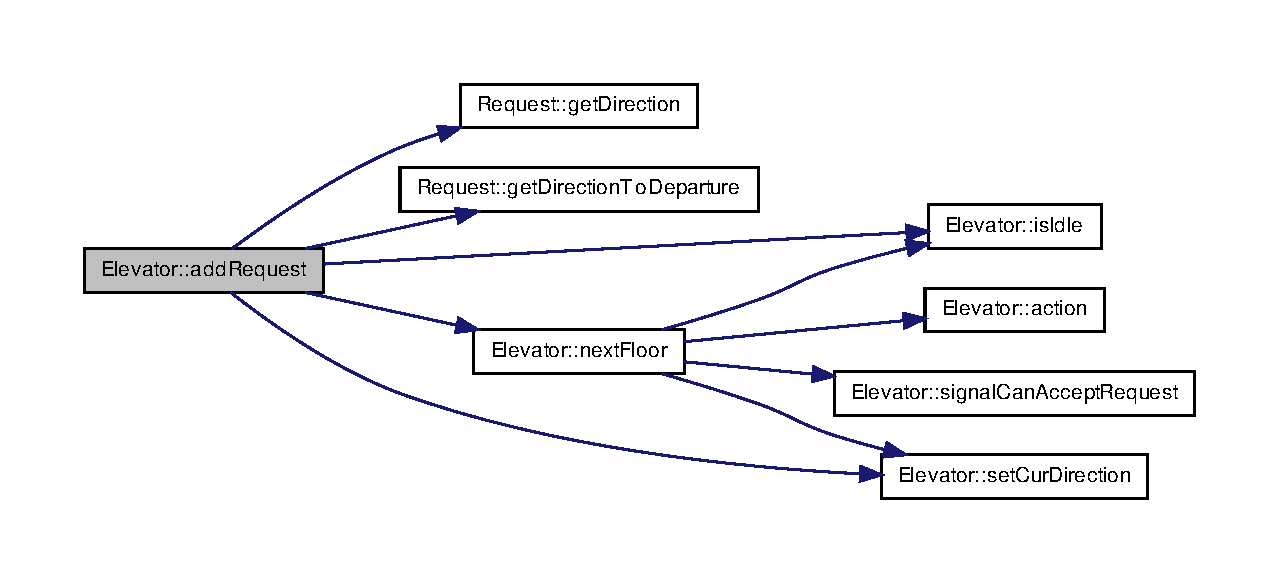
\includegraphics[width=400pt]{class_elevator_aaef88b9050a598bfc711e0f4a55711d0_cgraph}
\end{center}
\end{figure}




Here is the caller graph for this function:\nopagebreak
\begin{figure}[H]
\begin{center}
\leavevmode
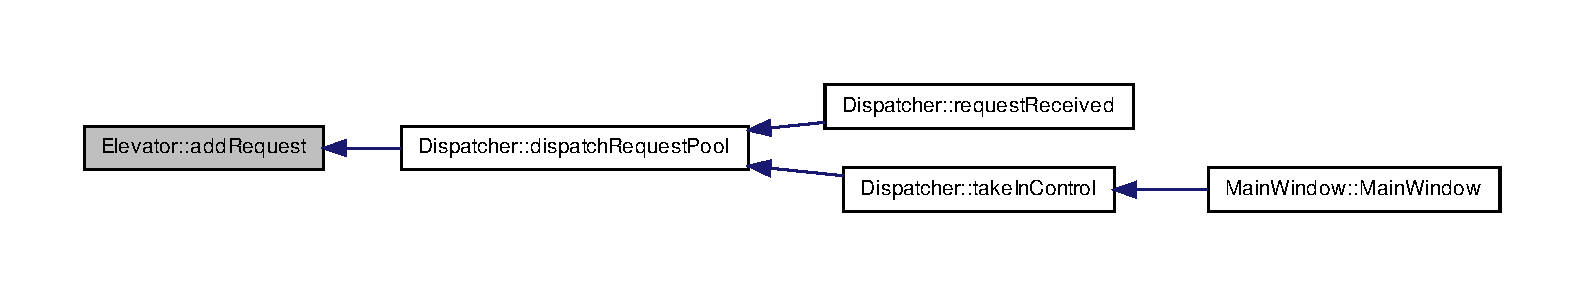
\includegraphics[width=400pt]{class_elevator_aaef88b9050a598bfc711e0f4a55711d0_icgraph}
\end{center}
\end{figure}


\hypertarget{class_elevator_a1c7640e845ad36870c764f87e53d21e2}{
\index{Elevator@{Elevator}!animeDoorOpenFinished@{animeDoorOpenFinished}}
\index{animeDoorOpenFinished@{animeDoorOpenFinished}!Elevator@{Elevator}}
\subsubsection[{animeDoorOpenFinished}]{\setlength{\rightskip}{0pt plus 5cm}void Elevator::animeDoorOpenFinished (
\begin{DoxyParamCaption}
{}
\end{DoxyParamCaption}
)\hspace{0.3cm}{\ttfamily  \mbox{[}inline, private, slot\mbox{]}}}}
\label{class_elevator_a1c7640e845ad36870c764f87e53d21e2}
Door has opened and show the animation target, then continue the animation 

Here is the caller graph for this function:\nopagebreak
\begin{figure}[H]
\begin{center}
\leavevmode
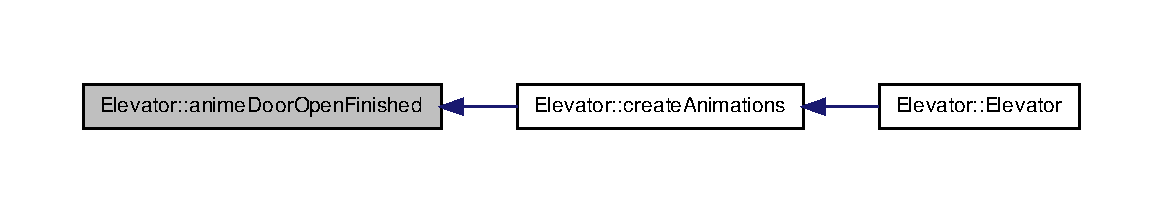
\includegraphics[width=400pt]{class_elevator_a1c7640e845ad36870c764f87e53d21e2_icgraph}
\end{center}
\end{figure}


\hypertarget{class_elevator_ad0d2554d24ea14d07afa2a7e5d00725a}{
\index{Elevator@{Elevator}!animePassengersFinished@{animePassengersFinished}}
\index{animePassengersFinished@{animePassengersFinished}!Elevator@{Elevator}}
\subsubsection[{animePassengersFinished}]{\setlength{\rightskip}{0pt plus 5cm}void Elevator::animePassengersFinished (
\begin{DoxyParamCaption}
{}
\end{DoxyParamCaption}
)\hspace{0.3cm}{\ttfamily  \mbox{[}inline, private, slot\mbox{]}}}}
\label{class_elevator_ad0d2554d24ea14d07afa2a7e5d00725a}
Dooe is going to close, hide the animation target, then play the door-\/close animation 

Here is the caller graph for this function:\nopagebreak
\begin{figure}[H]
\begin{center}
\leavevmode
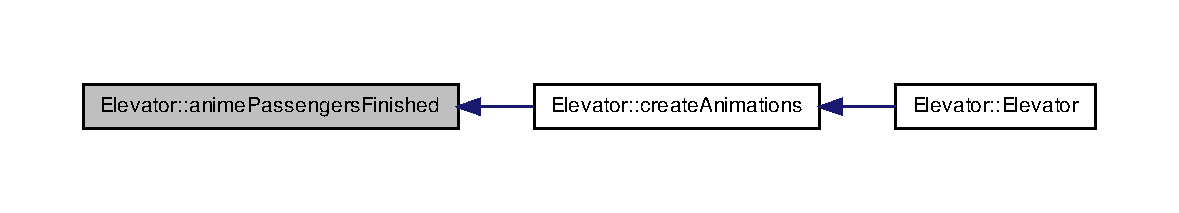
\includegraphics[width=400pt]{class_elevator_ad0d2554d24ea14d07afa2a7e5d00725a_icgraph}
\end{center}
\end{figure}


\hypertarget{class_elevator_a49c56159bb74facd0661c40f621b886f}{
\index{Elevator@{Elevator}!createAnimationDoor@{createAnimationDoor}}
\index{createAnimationDoor@{createAnimationDoor}!Elevator@{Elevator}}
\subsubsection[{createAnimationDoor}]{\setlength{\rightskip}{0pt plus 5cm}void Elevator::createAnimationDoor (
\begin{DoxyParamCaption}
{}
\end{DoxyParamCaption}
)\hspace{0.3cm}{\ttfamily  \mbox{[}inline, private\mbox{]}}}}
\label{class_elevator_a49c56159bb74facd0661c40f621b886f}
Create animations to open door, move passengers and close door 

Here is the caller graph for this function:\nopagebreak
\begin{figure}[H]
\begin{center}
\leavevmode
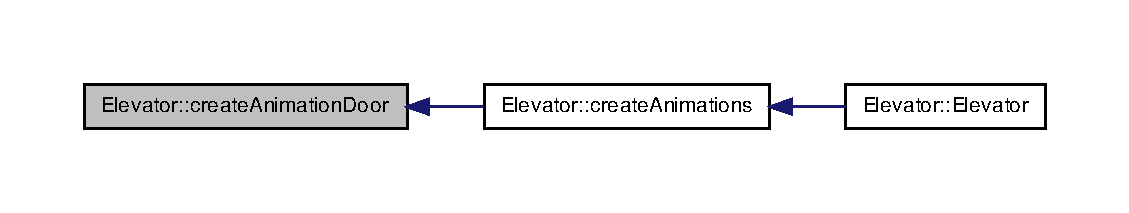
\includegraphics[width=400pt]{class_elevator_a49c56159bb74facd0661c40f621b886f_icgraph}
\end{center}
\end{figure}


\hypertarget{class_elevator_aabecded393aa00b30a1f2071b0ae1cdd}{
\index{Elevator@{Elevator}!createAnimationMove@{createAnimationMove}}
\index{createAnimationMove@{createAnimationMove}!Elevator@{Elevator}}
\subsubsection[{createAnimationMove}]{\setlength{\rightskip}{0pt plus 5cm}void Elevator::createAnimationMove (
\begin{DoxyParamCaption}
{}
\end{DoxyParamCaption}
)\hspace{0.3cm}{\ttfamily  \mbox{[}inline, private\mbox{]}}}}
\label{class_elevator_aabecded393aa00b30a1f2071b0ae1cdd}
Create animations to move elevator up and down 

Here is the caller graph for this function:\nopagebreak
\begin{figure}[H]
\begin{center}
\leavevmode
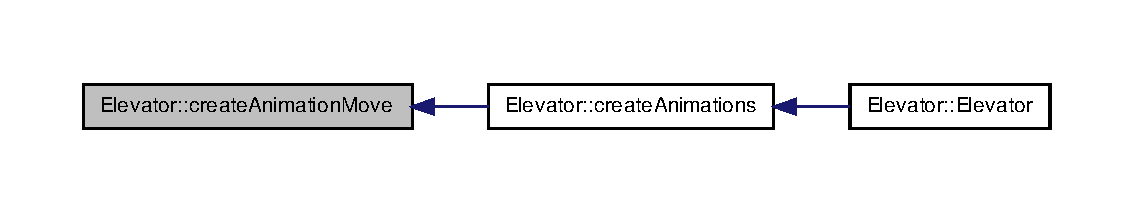
\includegraphics[width=400pt]{class_elevator_aabecded393aa00b30a1f2071b0ae1cdd_icgraph}
\end{center}
\end{figure}


\hypertarget{class_elevator_a92dbf1fd3ff98c4656ee428b43a35a4c}{
\index{Elevator@{Elevator}!createAnimations@{createAnimations}}
\index{createAnimations@{createAnimations}!Elevator@{Elevator}}
\subsubsection[{createAnimations}]{\setlength{\rightskip}{0pt plus 5cm}void Elevator::createAnimations (
\begin{DoxyParamCaption}
{}
\end{DoxyParamCaption}
)\hspace{0.3cm}{\ttfamily  \mbox{[}inline, private\mbox{]}}}}
\label{class_elevator_a92dbf1fd3ff98c4656ee428b43a35a4c}
Create and initialize the animations 

Here is the call graph for this function:\nopagebreak
\begin{figure}[H]
\begin{center}
\leavevmode
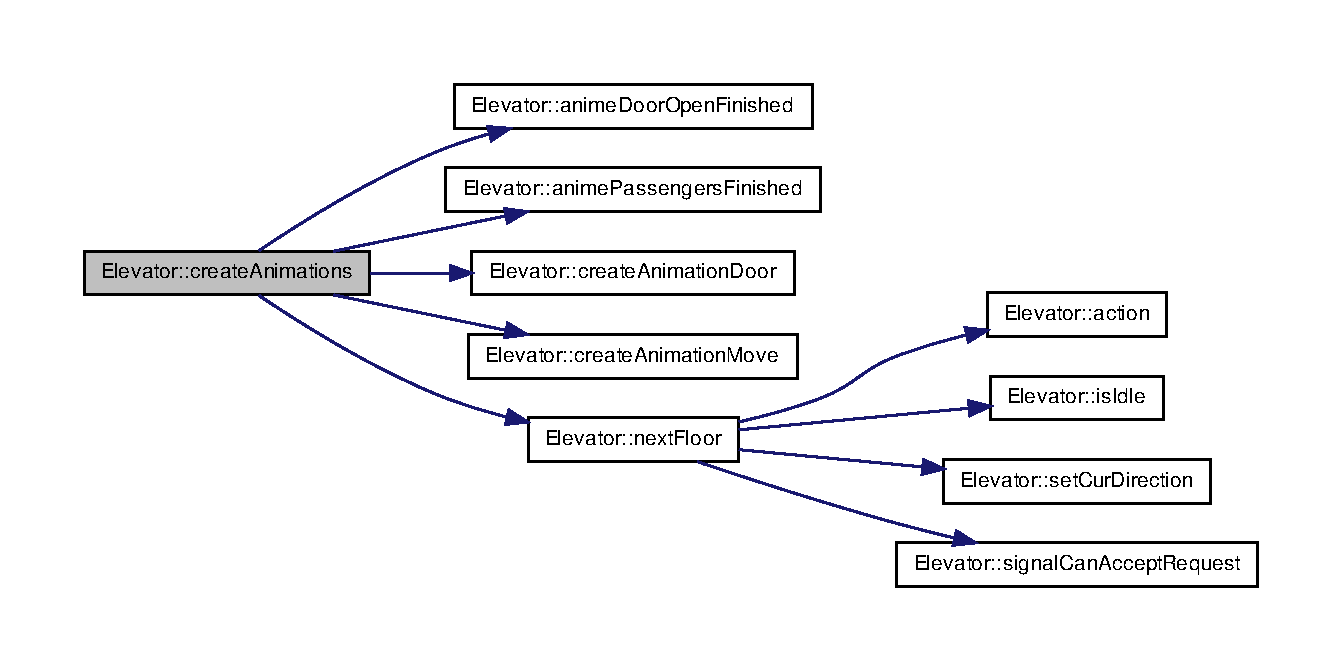
\includegraphics[width=400pt]{class_elevator_a92dbf1fd3ff98c4656ee428b43a35a4c_cgraph}
\end{center}
\end{figure}




Here is the caller graph for this function:\nopagebreak
\begin{figure}[H]
\begin{center}
\leavevmode
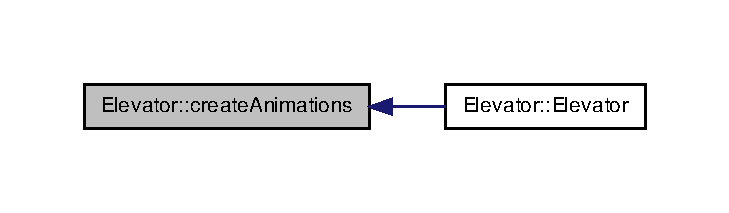
\includegraphics[width=350pt]{class_elevator_a92dbf1fd3ff98c4656ee428b43a35a4c_icgraph}
\end{center}
\end{figure}


\hypertarget{class_elevator_a2e9a499fe4d2b2ccff043d3798399743}{
\index{Elevator@{Elevator}!evaluate@{evaluate}}
\index{evaluate@{evaluate}!Elevator@{Elevator}}
\subsubsection[{evaluate}]{\setlength{\rightskip}{0pt plus 5cm}int Elevator::evaluate (
\begin{DoxyParamCaption}
\item[{{\bf Request} $\ast$}]{req}
\end{DoxyParamCaption}
)\hspace{0.3cm}{\ttfamily  \mbox{[}inline\mbox{]}}}}
\label{class_elevator_a2e9a499fe4d2b2ccff043d3798399743}
Evaluate whether a request can be accept by the elevator. If can, the function will return a int value representing the time that will cost to have the passenger arrived. If can't, REQUEST\_\-UNACCEPTABLE will be returned. 

Here is the call graph for this function:\nopagebreak
\begin{figure}[H]
\begin{center}
\leavevmode
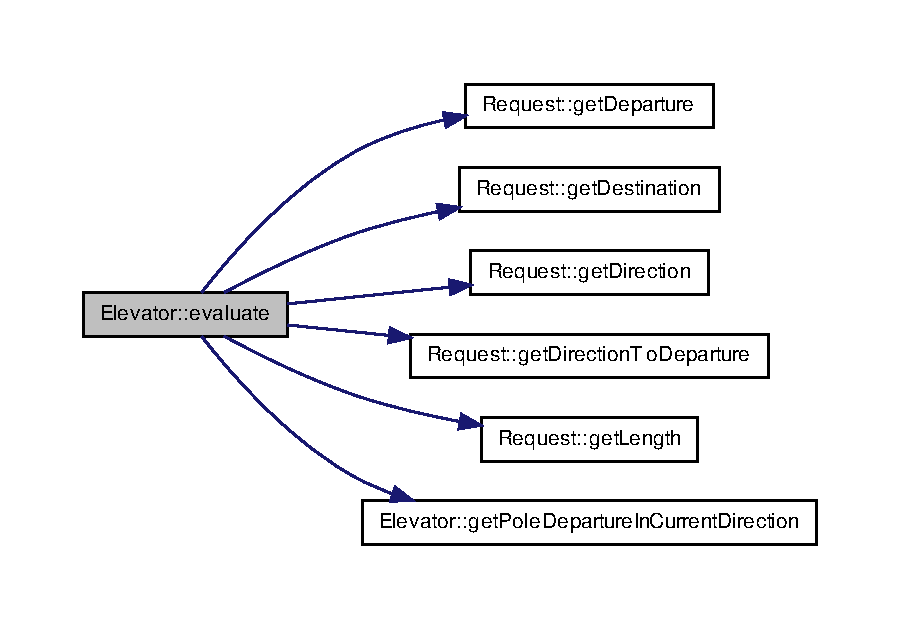
\includegraphics[width=400pt]{class_elevator_a2e9a499fe4d2b2ccff043d3798399743_cgraph}
\end{center}
\end{figure}




Here is the caller graph for this function:\nopagebreak
\begin{figure}[H]
\begin{center}
\leavevmode
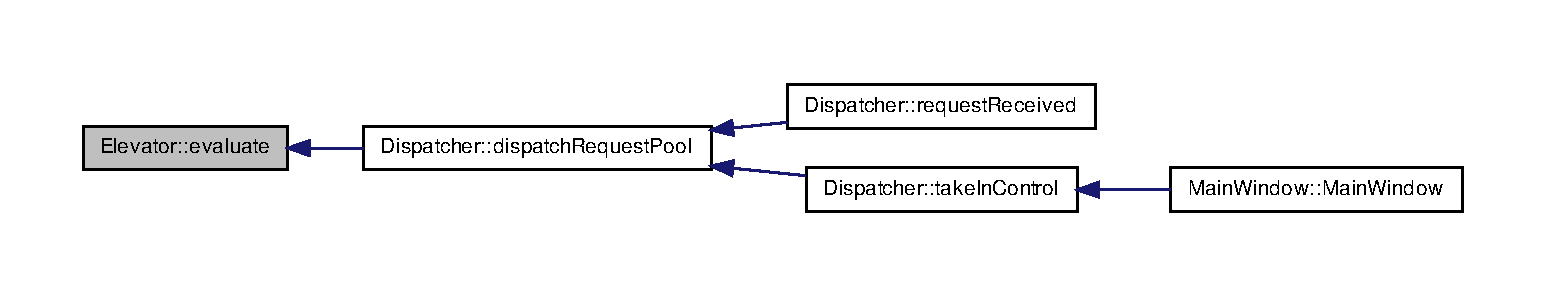
\includegraphics[width=400pt]{class_elevator_a2e9a499fe4d2b2ccff043d3798399743_icgraph}
\end{center}
\end{figure}


\hypertarget{class_elevator_a333ca5f86534823e1efda55e48c36abe}{
\index{Elevator@{Elevator}!getCurrentFloor@{getCurrentFloor}}
\index{getCurrentFloor@{getCurrentFloor}!Elevator@{Elevator}}
\subsubsection[{getCurrentFloor}]{\setlength{\rightskip}{0pt plus 5cm}int Elevator::getCurrentFloor (
\begin{DoxyParamCaption}
{}
\end{DoxyParamCaption}
)\hspace{0.3cm}{\ttfamily  \mbox{[}inline\mbox{]}}}}
\label{class_elevator_a333ca5f86534823e1efda55e48c36abe}
Return the floor number \hypertarget{class_elevator_aca5f48d0086a5791d6fa822c4efc4d96}{
\index{Elevator@{Elevator}!getID@{getID}}
\index{getID@{getID}!Elevator@{Elevator}}
\subsubsection[{getID}]{\setlength{\rightskip}{0pt plus 5cm}int Elevator::getID (
\begin{DoxyParamCaption}
{}
\end{DoxyParamCaption}
)\hspace{0.3cm}{\ttfamily  \mbox{[}inline\mbox{]}}}}
\label{class_elevator_aca5f48d0086a5791d6fa822c4efc4d96}
Return the ID(Index) of this \hyperlink{class_elevator}{Elevator} 

Here is the caller graph for this function:\nopagebreak
\begin{figure}[H]
\begin{center}
\leavevmode
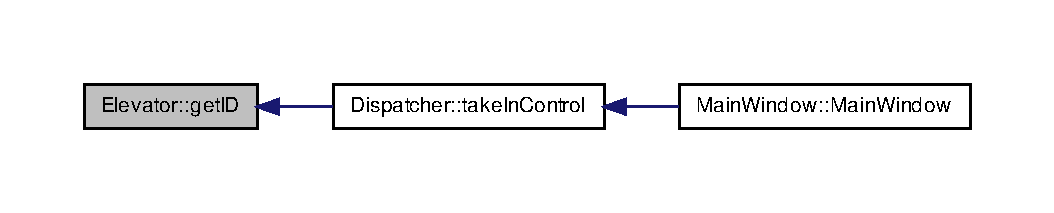
\includegraphics[width=400pt]{class_elevator_aca5f48d0086a5791d6fa822c4efc4d96_icgraph}
\end{center}
\end{figure}


\hypertarget{class_elevator_abd54853d9aba7177792df167c0bb894c}{
\index{Elevator@{Elevator}!getPoleDepartureInCurrentDirection@{getPoleDepartureInCurrentDirection}}
\index{getPoleDepartureInCurrentDirection@{getPoleDepartureInCurrentDirection}!Elevator@{Elevator}}
\subsubsection[{getPoleDepartureInCurrentDirection}]{\setlength{\rightskip}{0pt plus 5cm}int Elevator::getPoleDepartureInCurrentDirection (
\begin{DoxyParamCaption}
{}
\end{DoxyParamCaption}
)\hspace{0.3cm}{\ttfamily  \mbox{[}inline, private, slot\mbox{]}}}}
\label{class_elevator_abd54853d9aba7177792df167c0bb894c}
Get the pole value of the floor the \hyperlink{class_elevator}{Elevator} can arrived to take passengers along the current direction. 

Here is the caller graph for this function:\nopagebreak
\begin{figure}[H]
\begin{center}
\leavevmode
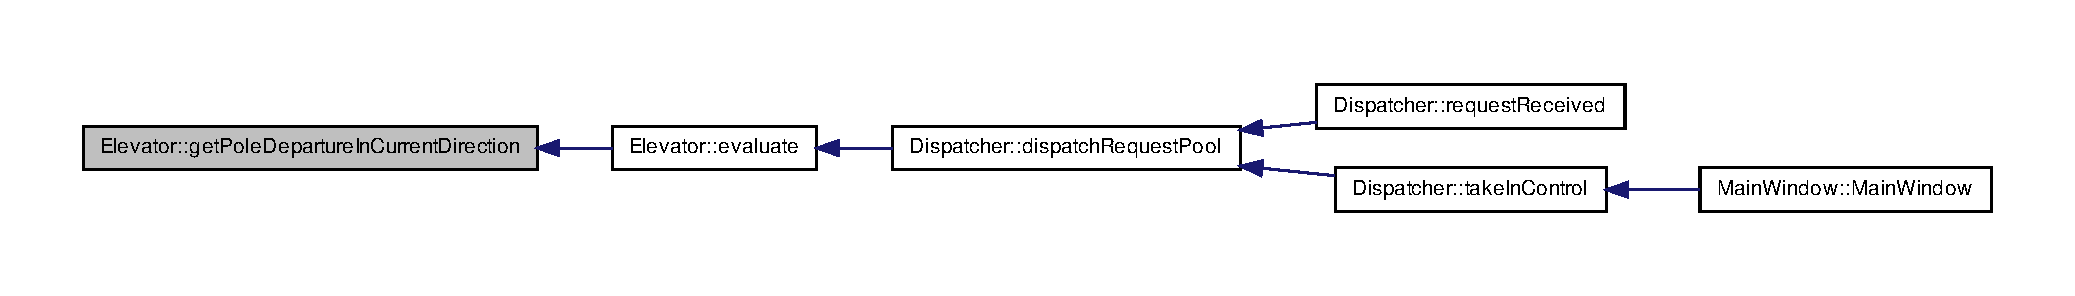
\includegraphics[width=400pt]{class_elevator_abd54853d9aba7177792df167c0bb894c_icgraph}
\end{center}
\end{figure}


\hypertarget{class_elevator_a64dc8a888c4ae8914a2ce640b3104c39}{
\index{Elevator@{Elevator}!isIdle@{isIdle}}
\index{isIdle@{isIdle}!Elevator@{Elevator}}
\subsubsection[{isIdle}]{\setlength{\rightskip}{0pt plus 5cm}bool Elevator::isIdle (
\begin{DoxyParamCaption}
{}
\end{DoxyParamCaption}
)\hspace{0.3cm}{\ttfamily  \mbox{[}inline\mbox{]}}}}
\label{class_elevator_a64dc8a888c4ae8914a2ce640b3104c39}
Return whether the elevator is idle 

Here is the caller graph for this function:\nopagebreak
\begin{figure}[H]
\begin{center}
\leavevmode
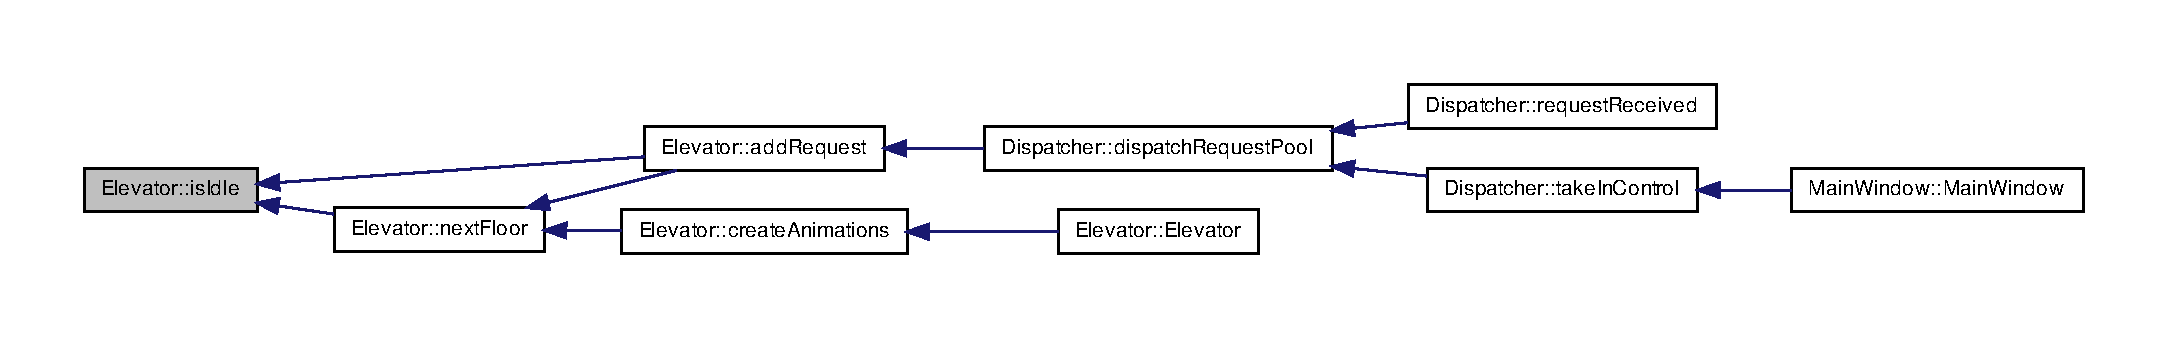
\includegraphics[width=400pt]{class_elevator_a64dc8a888c4ae8914a2ce640b3104c39_icgraph}
\end{center}
\end{figure}


\hypertarget{class_elevator_a5d4ecef44a3e87b14b5ce8de10008fdd}{
\index{Elevator@{Elevator}!nextFloor@{nextFloor}}
\index{nextFloor@{nextFloor}!Elevator@{Elevator}}
\subsubsection[{nextFloor}]{\setlength{\rightskip}{0pt plus 5cm}void Elevator::nextFloor (
\begin{DoxyParamCaption}
{}
\end{DoxyParamCaption}
)\hspace{0.3cm}{\ttfamily  \mbox{[}inline, private, slot\mbox{]}}}}
\label{class_elevator_a5d4ecef44a3e87b14b5ce8de10008fdd}
Core driver function for the running of the elevator. \par
 Control the curFloor, Open of the door, Passengers, Move of the \hyperlink{class_elevator}{Elevator}, Task List. 

Here is the call graph for this function:\nopagebreak
\begin{figure}[H]
\begin{center}
\leavevmode
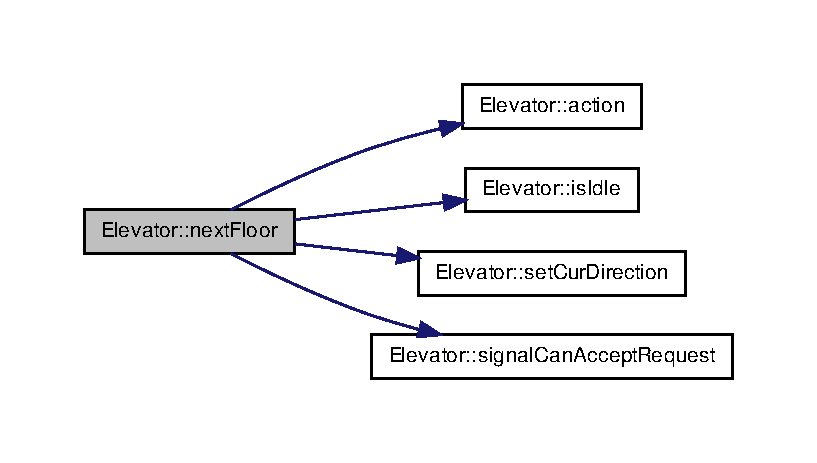
\includegraphics[width=392pt]{class_elevator_a5d4ecef44a3e87b14b5ce8de10008fdd_cgraph}
\end{center}
\end{figure}




Here is the caller graph for this function:\nopagebreak
\begin{figure}[H]
\begin{center}
\leavevmode
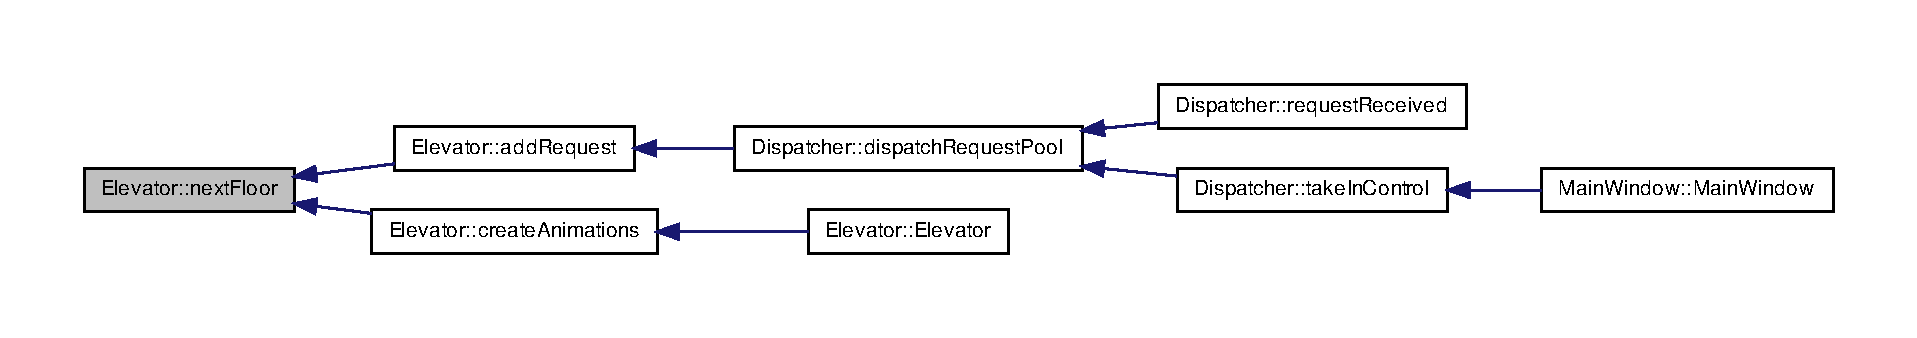
\includegraphics[width=400pt]{class_elevator_a5d4ecef44a3e87b14b5ce8de10008fdd_icgraph}
\end{center}
\end{figure}


\hypertarget{class_elevator_ad854f6f6fa0d4c8b6066edc1282fced3}{
\index{Elevator@{Elevator}!setCurDirection@{setCurDirection}}
\index{setCurDirection@{setCurDirection}!Elevator@{Elevator}}
\subsubsection[{setCurDirection}]{\setlength{\rightskip}{0pt plus 5cm}void Elevator::setCurDirection (
\begin{DoxyParamCaption}
\item[{{\bf Request::DIRECTION}}]{curDir}
\end{DoxyParamCaption}
)\hspace{0.3cm}{\ttfamily  \mbox{[}inline, private\mbox{]}}}}
\label{class_elevator_ad854f6f6fa0d4c8b6066edc1282fced3}
Set the current elevator direction to the given direction 

Here is the caller graph for this function:\nopagebreak
\begin{figure}[H]
\begin{center}
\leavevmode
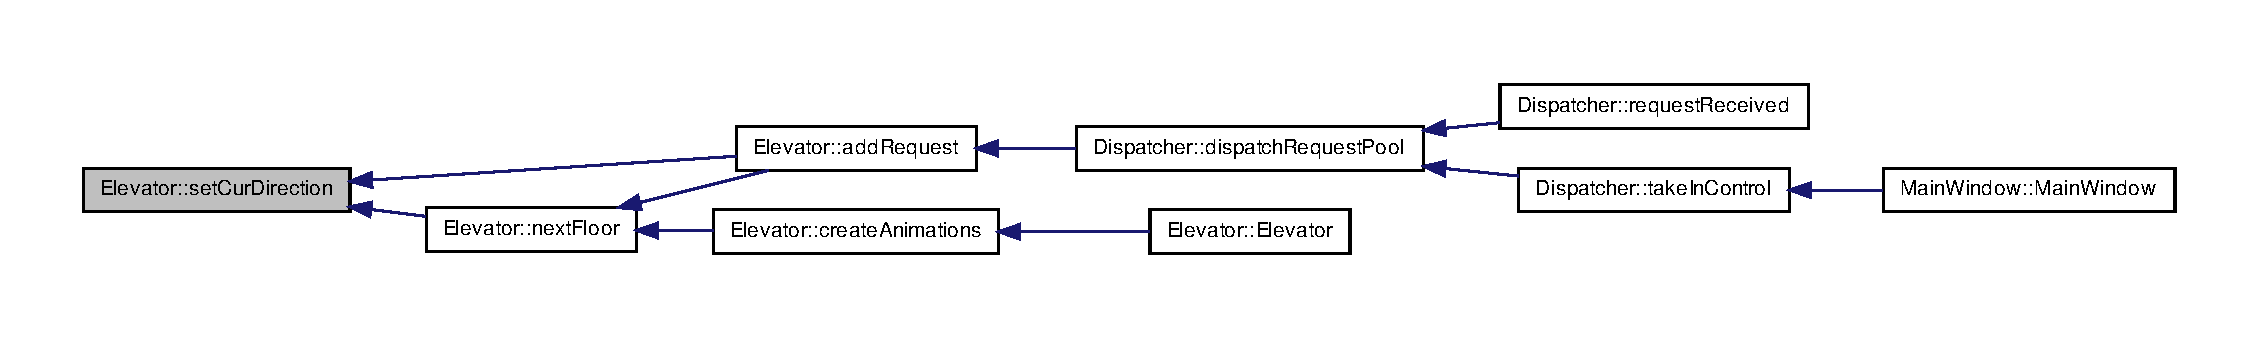
\includegraphics[width=400pt]{class_elevator_ad854f6f6fa0d4c8b6066edc1282fced3_icgraph}
\end{center}
\end{figure}


\hypertarget{class_elevator_a688a7f343cc5d4ceec45feea140ccba2}{
\index{Elevator@{Elevator}!signalCanAcceptRequest@{signalCanAcceptRequest}}
\index{signalCanAcceptRequest@{signalCanAcceptRequest}!Elevator@{Elevator}}
\subsubsection[{signalCanAcceptRequest}]{\setlength{\rightskip}{0pt plus 5cm}void Elevator::signalCanAcceptRequest (
\begin{DoxyParamCaption}
\item[{int}]{elevatorIndex}
\end{DoxyParamCaption}
)\hspace{0.3cm}{\ttfamily  \mbox{[}signal\mbox{]}}}}
\label{class_elevator_a688a7f343cc5d4ceec45feea140ccba2}
Signal sent when the elevator is idle or the direction of the elevator changed. 

Here is the caller graph for this function:\nopagebreak
\begin{figure}[H]
\begin{center}
\leavevmode
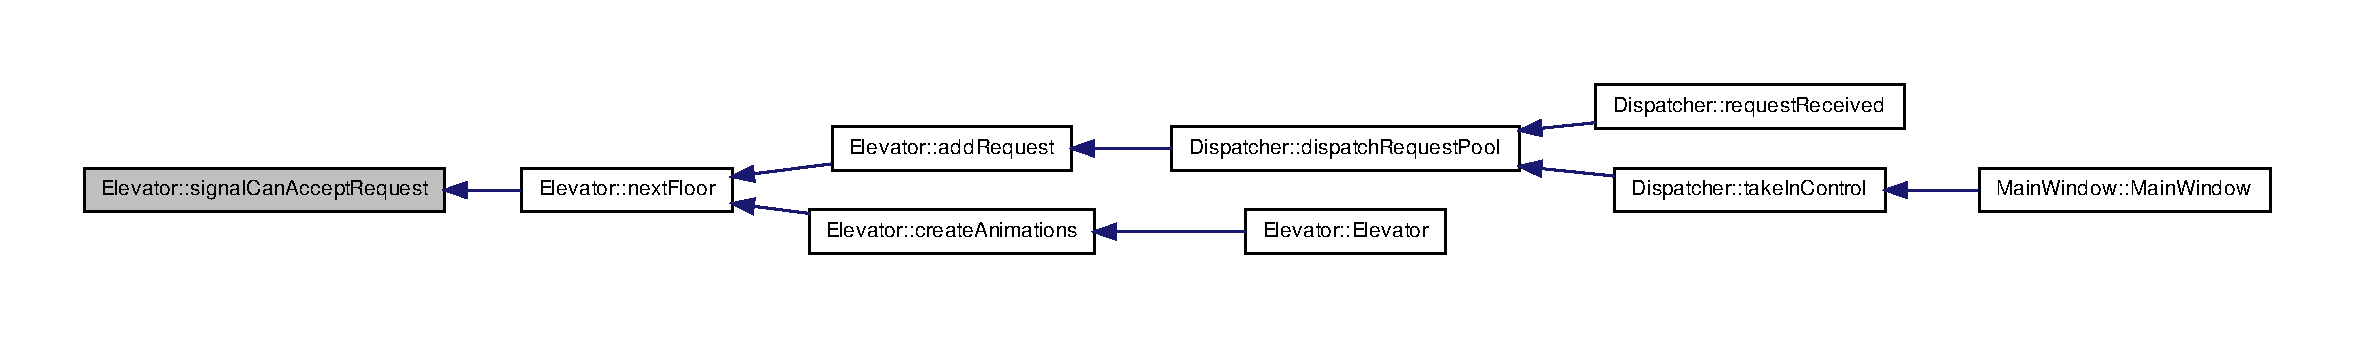
\includegraphics[width=400pt]{class_elevator_a688a7f343cc5d4ceec45feea140ccba2_icgraph}
\end{center}
\end{figure}




The documentation for this class was generated from the following files:\begin{DoxyCompactItemize}
\item 
elevator.h\item 
main.cpp\end{DoxyCompactItemize}

\hypertarget{class_main_window}{
\section{MainWindow Class Reference}
\label{class_main_window}\index{MainWindow@{MainWindow}}
}


{\ttfamily \#include $<$mainwindow.h$>$}



Collaboration diagram for MainWindow:\nopagebreak
\begin{figure}[H]
\begin{center}
\leavevmode
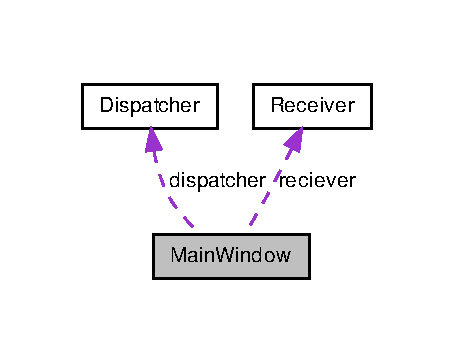
\includegraphics[width=218pt]{class_main_window__coll__graph}
\end{center}
\end{figure}
\subsection*{Public Member Functions}
\begin{DoxyCompactItemize}
\item 
\hyperlink{class_main_window_a8b244be8b7b7db1b08de2a2acb9409db}{MainWindow} (QWidget $\ast$parent=0)
\end{DoxyCompactItemize}
\subsection*{Private Attributes}
\begin{DoxyCompactItemize}
\item 
\hypertarget{class_main_window_a49a4cc5b54e6219a3184e835d55ea15b}{
Ui::SimElevators \hyperlink{class_main_window_a49a4cc5b54e6219a3184e835d55ea15b}{ui}}
\label{class_main_window_a49a4cc5b54e6219a3184e835d55ea15b}

\begin{DoxyCompactList}\small\item\em Qt UI object. \end{DoxyCompactList}\item 
\hypertarget{class_main_window_ab3d26981023f4d64c8fab3faeb0743b1}{
\hyperlink{class_dispatcher}{Dispatcher} $\ast$ \hyperlink{class_main_window_ab3d26981023f4d64c8fab3faeb0743b1}{dispatcher}}
\label{class_main_window_ab3d26981023f4d64c8fab3faeb0743b1}

\begin{DoxyCompactList}\small\item\em Request-\/Dispatcher object. \end{DoxyCompactList}\item 
\hypertarget{class_main_window_a7c9432520c16d148bd426e93b8c86383}{
\hyperlink{class_receiver}{Receiver} $\ast$ \hyperlink{class_main_window_a7c9432520c16d148bd426e93b8c86383}{reciever}}
\label{class_main_window_a7c9432520c16d148bd426e93b8c86383}

\begin{DoxyCompactList}\small\item\em Request-\/Receiver object. \end{DoxyCompactList}\end{DoxyCompactItemize}


\subsection{Detailed Description}
Main Window Class 

\subsection{Constructor \& Destructor Documentation}
\hypertarget{class_main_window_a8b244be8b7b7db1b08de2a2acb9409db}{
\index{MainWindow@{MainWindow}!MainWindow@{MainWindow}}
\index{MainWindow@{MainWindow}!MainWindow@{MainWindow}}
\subsubsection[{MainWindow}]{\setlength{\rightskip}{0pt plus 5cm}MainWindow::MainWindow (
\begin{DoxyParamCaption}
\item[{QWidget $\ast$}]{parent = {\ttfamily 0}}
\end{DoxyParamCaption}
)\hspace{0.3cm}{\ttfamily  \mbox{[}inline, explicit\mbox{]}}}}
\label{class_main_window_a8b244be8b7b7db1b08de2a2acb9409db}
Constructor for Main Window. Initialize a \hyperlink{class_dispatcher}{Dispatcher} and Reciever. Have all the \hyperlink{class_elevator}{Elevator} widgets on ui connected to \hyperlink{class_dispatcher}{Dispatcher}. Connect the Reciever to \hyperlink{class_dispatcher}{Dispatcher}. 

Here is the call graph for this function:\nopagebreak
\begin{figure}[H]
\begin{center}
\leavevmode
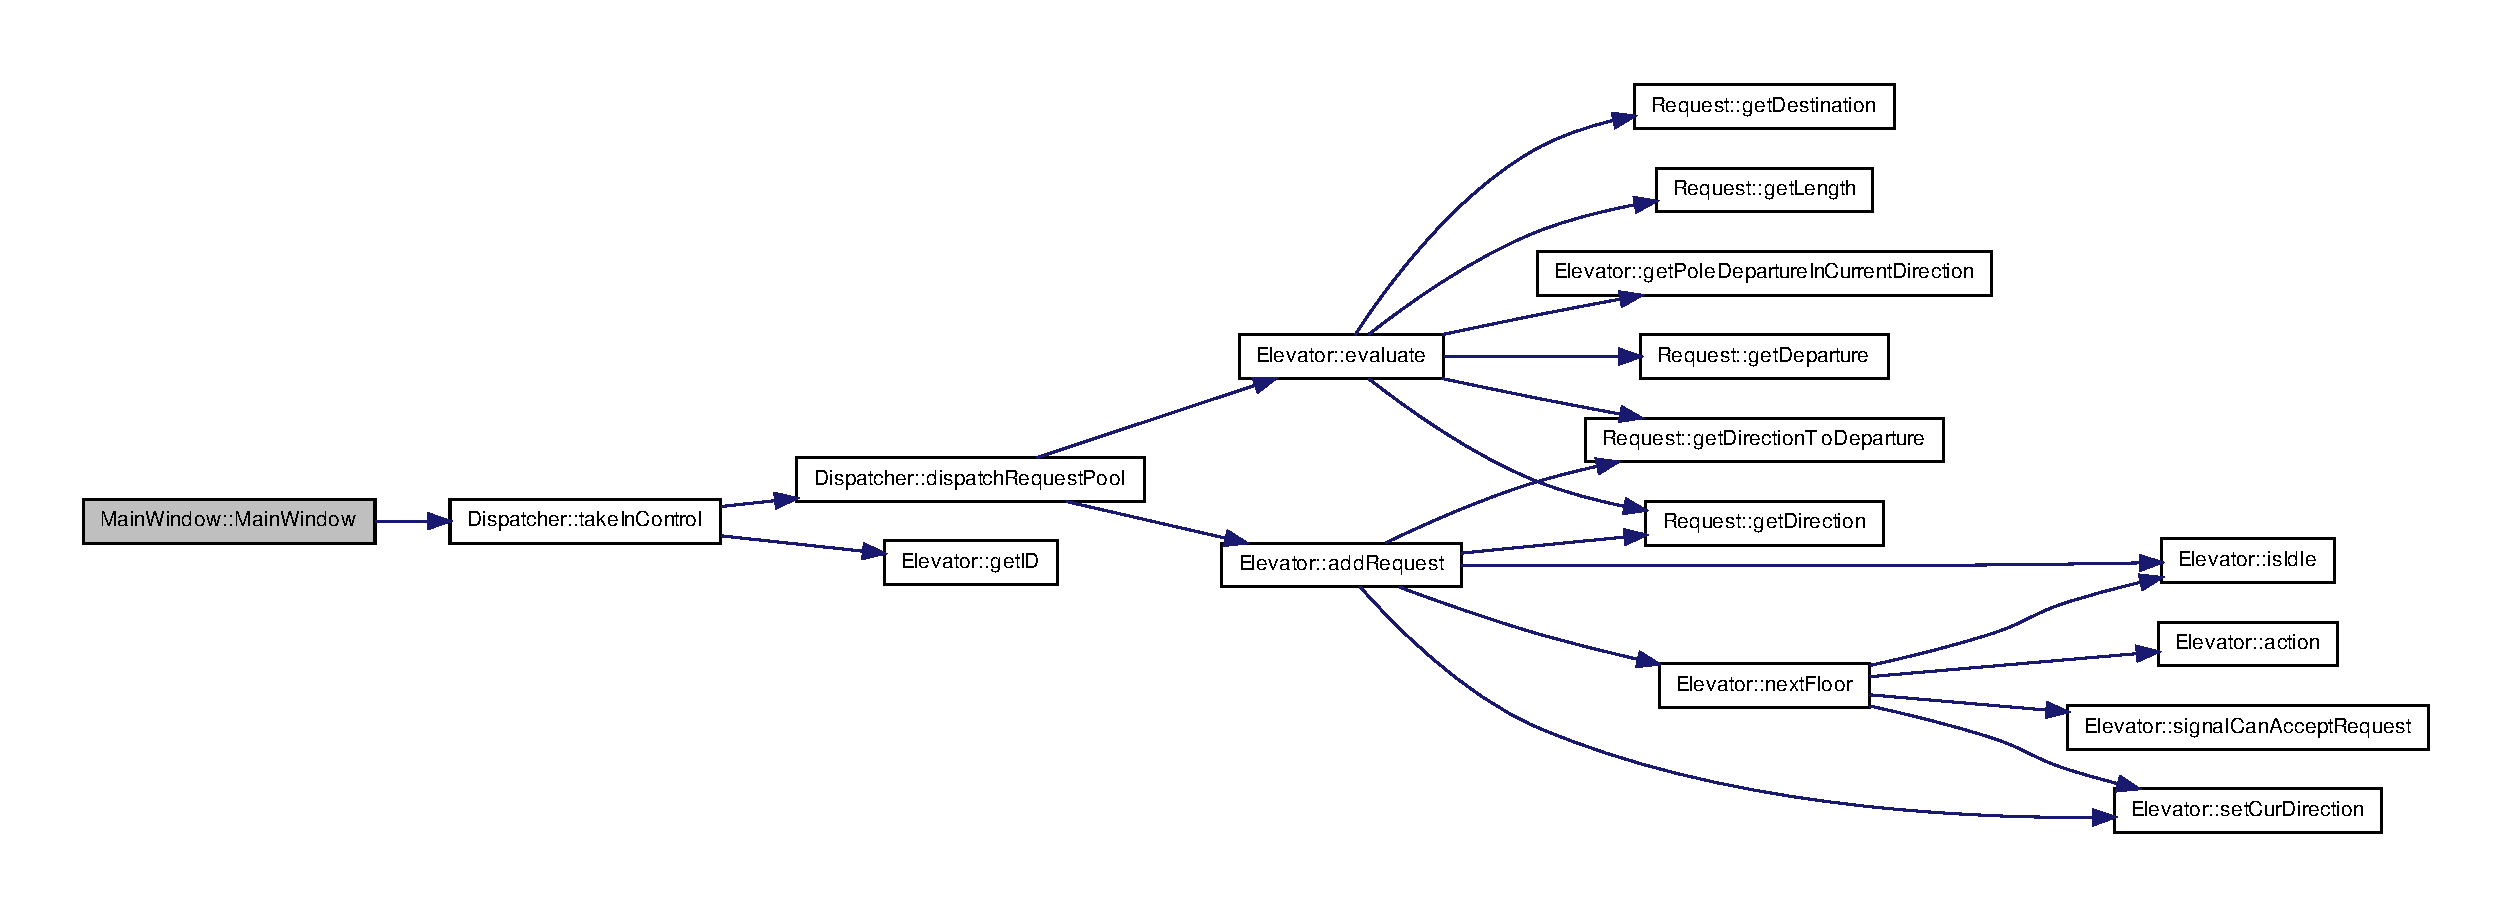
\includegraphics[width=400pt]{class_main_window_a8b244be8b7b7db1b08de2a2acb9409db_cgraph}
\end{center}
\end{figure}




The documentation for this class was generated from the following file:\begin{DoxyCompactItemize}
\item 
mainwindow.h\end{DoxyCompactItemize}

\hypertarget{class_receiver}{
\section{Receiver Class Reference}
\label{class_receiver}\index{Receiver@{Receiver}}
}


{\ttfamily \#include $<$receiver.h$>$}

\subsection*{Signals}
\begin{DoxyCompactItemize}
\item 
void \hyperlink{class_receiver_a1d7579bc5666c14449f5986d6fd26e7d}{signalRequestReceived} (\hyperlink{class_request}{Request} $\ast$req)
\end{DoxyCompactItemize}
\subsection*{Public Member Functions}
\begin{DoxyCompactItemize}
\item 
\hyperlink{class_receiver_af9c313fb6638894c3e31f6ed93684728}{Receiver} (QObject $\ast$parent=0)
\item 
void \hyperlink{class_receiver_a4e4b7449e28362cdfeb05c349f6d1888}{incomingConnection} (int socket)
\end{DoxyCompactItemize}
\subsection*{Static Public Attributes}
\begin{DoxyCompactItemize}
\item 
static const int \hyperlink{class_receiver_a9960b604c1574e1d5876aeef979addfd}{UPPER\_\-FLOOR} = 50
\end{DoxyCompactItemize}
\subsection*{Private Slots}
\begin{DoxyCompactItemize}
\item 
void \hyperlink{class_receiver_a48b94424274f0d0fc2a3bbee87aaa25c}{readClient} ()
\item 
\hypertarget{class_receiver_a0a7a8e1194211358e027e3ada7cfdb36}{
void {\bfseries discardClient} ()}
\label{class_receiver_a0a7a8e1194211358e027e3ada7cfdb36}

\end{DoxyCompactItemize}


\subsection{Detailed Description}
\hyperlink{class_receiver}{Receiver} Object Run in HTTP Server Mode, Listen for requests on port 8369 

\subsection{Constructor \& Destructor Documentation}
\hypertarget{class_receiver_af9c313fb6638894c3e31f6ed93684728}{
\index{Receiver@{Receiver}!Receiver@{Receiver}}
\index{Receiver@{Receiver}!Receiver@{Receiver}}
\subsubsection[{Receiver}]{\setlength{\rightskip}{0pt plus 5cm}Receiver::Receiver (
\begin{DoxyParamCaption}
\item[{QObject $\ast$}]{parent = {\ttfamily 0}}
\end{DoxyParamCaption}
)\hspace{0.3cm}{\ttfamily  \mbox{[}inline\mbox{]}}}}
\label{class_receiver_af9c313fb6638894c3e31f6ed93684728}
Start the listening of the HTTP server, if port is taken no error will be reported. 

\subsection{Member Function Documentation}
\hypertarget{class_receiver_a4e4b7449e28362cdfeb05c349f6d1888}{
\index{Receiver@{Receiver}!incomingConnection@{incomingConnection}}
\index{incomingConnection@{incomingConnection}!Receiver@{Receiver}}
\subsubsection[{incomingConnection}]{\setlength{\rightskip}{0pt plus 5cm}void Receiver::incomingConnection (
\begin{DoxyParamCaption}
\item[{int}]{socket}
\end{DoxyParamCaption}
)\hspace{0.3cm}{\ttfamily  \mbox{[}inline\mbox{]}}}}
\label{class_receiver_a4e4b7449e28362cdfeb05c349f6d1888}
Function triggered when a connection request is in. Accept the connection and forward it to the slot readClient. 

Here is the call graph for this function:\nopagebreak
\begin{figure}[H]
\begin{center}
\leavevmode
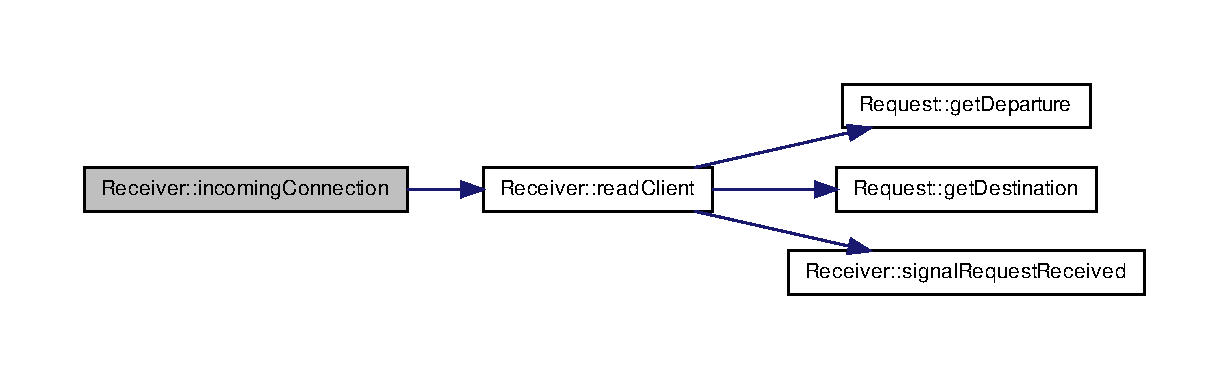
\includegraphics[width=400pt]{class_receiver_a4e4b7449e28362cdfeb05c349f6d1888_cgraph}
\end{center}
\end{figure}


\hypertarget{class_receiver_a48b94424274f0d0fc2a3bbee87aaa25c}{
\index{Receiver@{Receiver}!readClient@{readClient}}
\index{readClient@{readClient}!Receiver@{Receiver}}
\subsubsection[{readClient}]{\setlength{\rightskip}{0pt plus 5cm}void Receiver::readClient (
\begin{DoxyParamCaption}
{}
\end{DoxyParamCaption}
)\hspace{0.3cm}{\ttfamily  \mbox{[}inline, private, slot\mbox{]}}}}
\label{class_receiver_a48b94424274f0d0fc2a3bbee87aaa25c}
Slot to parse the received data to request and return message for client. 

Here is the call graph for this function:\nopagebreak
\begin{figure}[H]
\begin{center}
\leavevmode
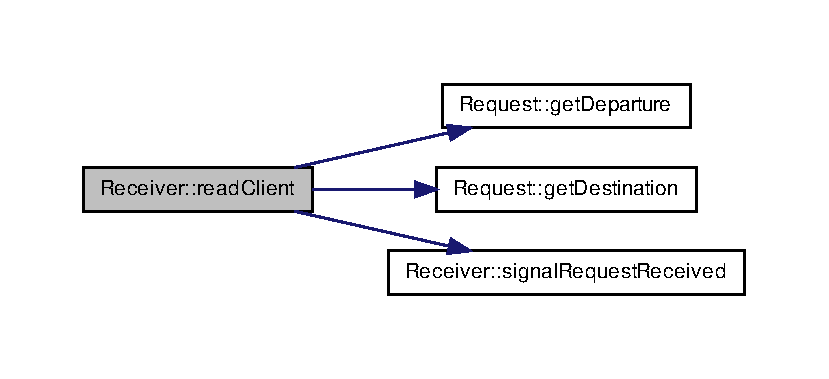
\includegraphics[width=398pt]{class_receiver_a48b94424274f0d0fc2a3bbee87aaa25c_cgraph}
\end{center}
\end{figure}




Here is the caller graph for this function:\nopagebreak
\begin{figure}[H]
\begin{center}
\leavevmode
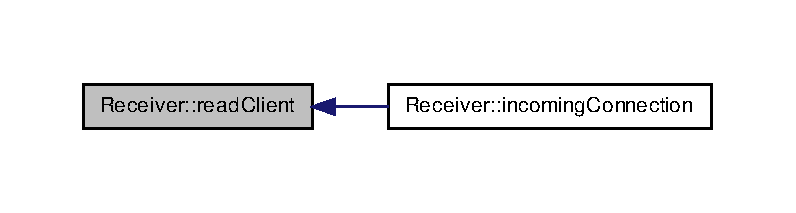
\includegraphics[width=382pt]{class_receiver_a48b94424274f0d0fc2a3bbee87aaa25c_icgraph}
\end{center}
\end{figure}


\hypertarget{class_receiver_a1d7579bc5666c14449f5986d6fd26e7d}{
\index{Receiver@{Receiver}!signalRequestReceived@{signalRequestReceived}}
\index{signalRequestReceived@{signalRequestReceived}!Receiver@{Receiver}}
\subsubsection[{signalRequestReceived}]{\setlength{\rightskip}{0pt plus 5cm}void Receiver::signalRequestReceived (
\begin{DoxyParamCaption}
\item[{{\bf Request} $\ast$}]{req}
\end{DoxyParamCaption}
)\hspace{0.3cm}{\ttfamily  \mbox{[}signal\mbox{]}}}}
\label{class_receiver_a1d7579bc5666c14449f5986d6fd26e7d}
Function triggered when an avaliable is received. 

Here is the caller graph for this function:\nopagebreak
\begin{figure}[H]
\begin{center}
\leavevmode
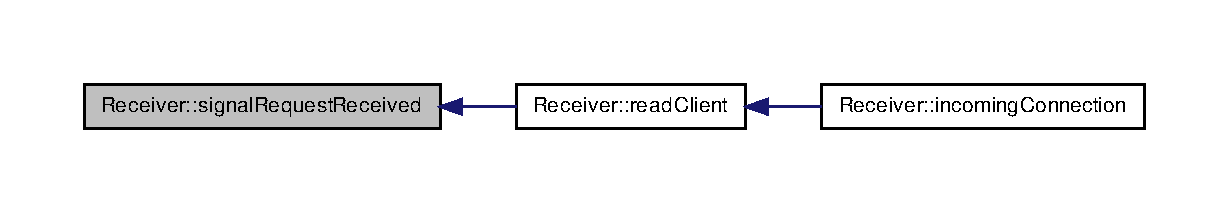
\includegraphics[width=400pt]{class_receiver_a1d7579bc5666c14449f5986d6fd26e7d_icgraph}
\end{center}
\end{figure}




\subsection{Member Data Documentation}
\hypertarget{class_receiver_a9960b604c1574e1d5876aeef979addfd}{
\index{Receiver@{Receiver}!UPPER\_\-FLOOR@{UPPER\_\-FLOOR}}
\index{UPPER\_\-FLOOR@{UPPER\_\-FLOOR}!Receiver@{Receiver}}
\subsubsection[{UPPER\_\-FLOOR}]{\setlength{\rightskip}{0pt plus 5cm}const int {\bf Receiver::UPPER\_\-FLOOR} = 50\hspace{0.3cm}{\ttfamily  \mbox{[}static\mbox{]}}}}
\label{class_receiver_a9960b604c1574e1d5876aeef979addfd}
Maxmum floor The request may reach 

The documentation for this class was generated from the following file:\begin{DoxyCompactItemize}
\item 
receiver.h\end{DoxyCompactItemize}

\hypertarget{class_request}{
\section{Request Class Reference}
\label{class_request}\index{Request@{Request}}
}


{\ttfamily \#include $<$request.h$>$}

\subsection*{Public Types}
\begin{DoxyCompactItemize}
\item 
enum \hyperlink{class_request_a31872cb7919df688dc6866ea607b9d9d}{DIRECTION} \{ {\bfseries DIRECTION\_\-UP}, 
{\bfseries DIRECTION\_\-DOWN}, 
{\bfseries DIRECTION\_\-NONE}
 \}
\end{DoxyCompactItemize}
\subsection*{Public Member Functions}
\begin{DoxyCompactItemize}
\item 
\hyperlink{class_request_a65d1a250d302018d1211fbdb2b8e0345}{Request} (int f, int t)
\item 
void \hyperlink{class_request_a76a1f5a44df4120828d34a90fbcec13e}{unsetDeparture} ()
\item 
void \hyperlink{class_request_addbd9fdcd5e5a0291c89aad38f6c8416}{unsetDestination} ()
\item 
int \hyperlink{class_request_a7199b71072973cac67be00225bd9ce5b}{getDeparture} ()
\item 
int \hyperlink{class_request_af8586495f2fd5dce9fc5690d47f59310}{getDestination} ()
\item 
int \hyperlink{class_request_a78b24de8cdef27ff340b28d49d251720}{getLength} ()
\item 
\hyperlink{class_request_a31872cb7919df688dc6866ea607b9d9d}{DIRECTION} \hyperlink{class_request_af75b4fec08458a4fe539d679d87ac8c4}{getDirection} ()
\item 
\hyperlink{class_request_a31872cb7919df688dc6866ea607b9d9d}{DIRECTION} \hyperlink{class_request_a7a435c886ed19acb556dc2445a53bd37}{getDirectionToDeparture} (int floor)
\item 
\hyperlink{class_request_a31872cb7919df688dc6866ea607b9d9d}{DIRECTION} \hyperlink{class_request_aeae53642527adaf40498ec5b05921ca0}{getDirectionToDestination} (int floor)
\end{DoxyCompactItemize}
\subsection*{Static Public Attributes}
\begin{DoxyCompactItemize}
\item 
static const int \hyperlink{class_request_a9bf9e694beed6b73dd9eaf3f3a73708b}{FLOOR\_\-NONE} = -\/1
\end{DoxyCompactItemize}
\subsection*{Private Attributes}
\begin{DoxyCompactItemize}
\item 
\hypertarget{class_request_a485c04f740b2b104773e7a562490daa9}{
int \hyperlink{class_request_a485c04f740b2b104773e7a562490daa9}{departure}}
\label{class_request_a485c04f740b2b104773e7a562490daa9}

\begin{DoxyCompactList}\small\item\em Variable to store the departure floor. \end{DoxyCompactList}\item 
\hypertarget{class_request_a4f515d80c8c978b213af816b54598497}{
int \hyperlink{class_request_a4f515d80c8c978b213af816b54598497}{destination}}
\label{class_request_a4f515d80c8c978b213af816b54598497}

\begin{DoxyCompactList}\small\item\em Variable to store the destination floor. \end{DoxyCompactList}\end{DoxyCompactItemize}


\subsection{Detailed Description}
\hyperlink{class_request}{Request} Class A \hyperlink{class_request}{Request} submitted by the passenger with where the passenger depart and where to arrive 

\subsection{Member Enumeration Documentation}
\hypertarget{class_request_a31872cb7919df688dc6866ea607b9d9d}{
\index{Request@{Request}!DIRECTION@{DIRECTION}}
\index{DIRECTION@{DIRECTION}!Request@{Request}}
\subsubsection[{DIRECTION}]{\setlength{\rightskip}{0pt plus 5cm}enum {\bf Request::DIRECTION}}}
\label{class_request_a31872cb7919df688dc6866ea607b9d9d}
Directions which the elevator will go 

\subsection{Constructor \& Destructor Documentation}
\hypertarget{class_request_a65d1a250d302018d1211fbdb2b8e0345}{
\index{Request@{Request}!Request@{Request}}
\index{Request@{Request}!Request@{Request}}
\subsubsection[{Request}]{\setlength{\rightskip}{0pt plus 5cm}Request::Request (
\begin{DoxyParamCaption}
\item[{int}]{f, }
\item[{int}]{t}
\end{DoxyParamCaption}
)\hspace{0.3cm}{\ttfamily  \mbox{[}inline\mbox{]}}}}
\label{class_request_a65d1a250d302018d1211fbdb2b8e0345}
Construct a \hyperlink{class_request}{Request} Class with the 'from' and 'to' param 

\subsection{Member Function Documentation}
\hypertarget{class_request_a7199b71072973cac67be00225bd9ce5b}{
\index{Request@{Request}!getDeparture@{getDeparture}}
\index{getDeparture@{getDeparture}!Request@{Request}}
\subsubsection[{getDeparture}]{\setlength{\rightskip}{0pt plus 5cm}int Request::getDeparture (
\begin{DoxyParamCaption}
{}
\end{DoxyParamCaption}
)\hspace{0.3cm}{\ttfamily  \mbox{[}inline\mbox{]}}}}
\label{class_request_a7199b71072973cac67be00225bd9ce5b}
Get the Departure floor from 1 to +INF and FLOOR\_\-NONE. 

Here is the caller graph for this function:\nopagebreak
\begin{figure}[H]
\begin{center}
\leavevmode
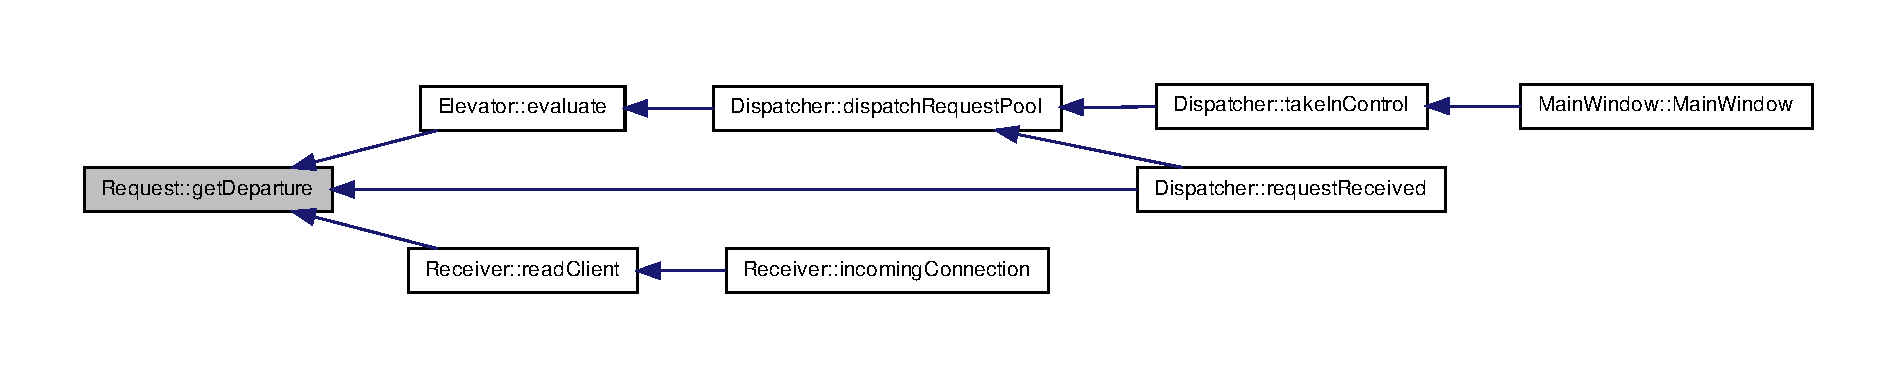
\includegraphics[width=400pt]{class_request_a7199b71072973cac67be00225bd9ce5b_icgraph}
\end{center}
\end{figure}


\hypertarget{class_request_af8586495f2fd5dce9fc5690d47f59310}{
\index{Request@{Request}!getDestination@{getDestination}}
\index{getDestination@{getDestination}!Request@{Request}}
\subsubsection[{getDestination}]{\setlength{\rightskip}{0pt plus 5cm}int Request::getDestination (
\begin{DoxyParamCaption}
{}
\end{DoxyParamCaption}
)\hspace{0.3cm}{\ttfamily  \mbox{[}inline\mbox{]}}}}
\label{class_request_af8586495f2fd5dce9fc5690d47f59310}
Get the Destination floor from 1 to +INF and FLOOR\_\-NONE. 

Here is the caller graph for this function:\nopagebreak
\begin{figure}[H]
\begin{center}
\leavevmode
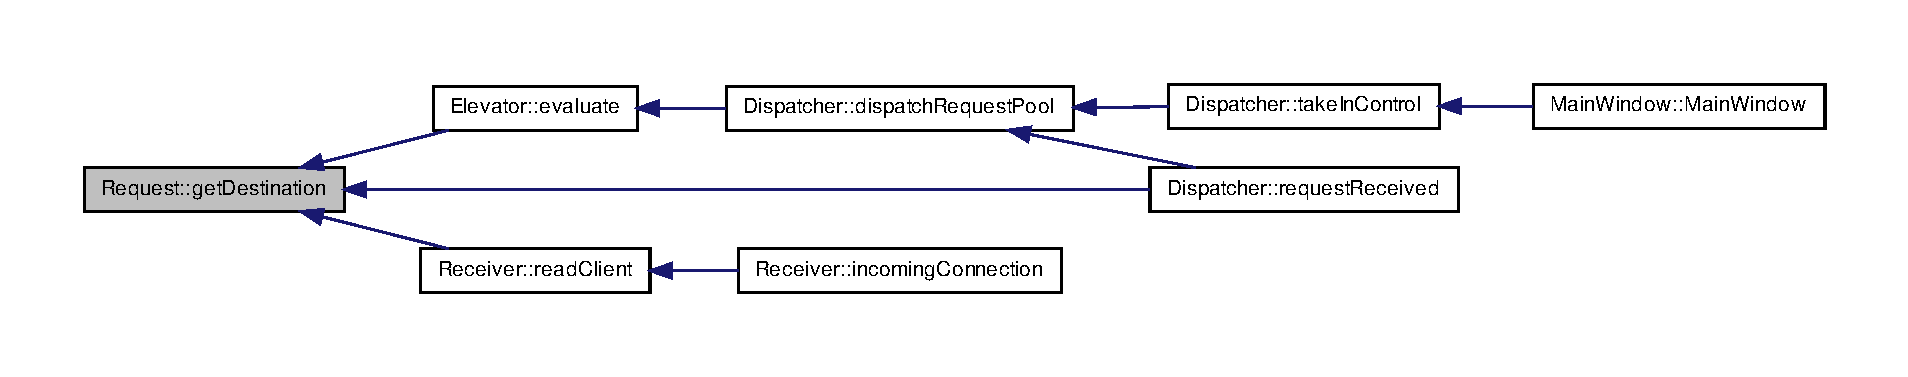
\includegraphics[width=400pt]{class_request_af8586495f2fd5dce9fc5690d47f59310_icgraph}
\end{center}
\end{figure}


\hypertarget{class_request_af75b4fec08458a4fe539d679d87ac8c4}{
\index{Request@{Request}!getDirection@{getDirection}}
\index{getDirection@{getDirection}!Request@{Request}}
\subsubsection[{getDirection}]{\setlength{\rightskip}{0pt plus 5cm}{\bf DIRECTION} Request::getDirection (
\begin{DoxyParamCaption}
{}
\end{DoxyParamCaption}
)\hspace{0.3cm}{\ttfamily  \mbox{[}inline\mbox{]}}}}
\label{class_request_af75b4fec08458a4fe539d679d87ac8c4}
Get the the DIRECTION from departure floor to destiination floor. 

Here is the caller graph for this function:\nopagebreak
\begin{figure}[H]
\begin{center}
\leavevmode
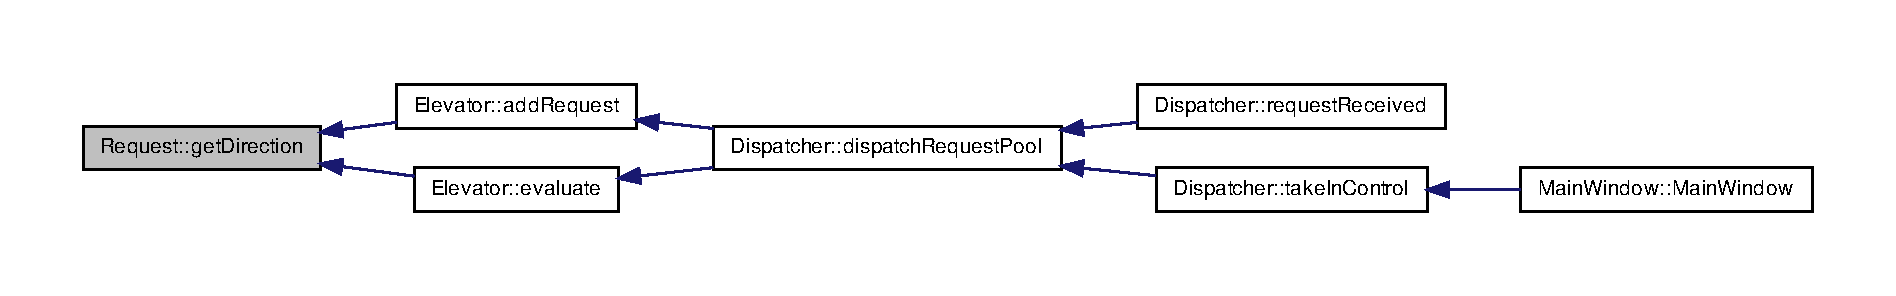
\includegraphics[width=400pt]{class_request_af75b4fec08458a4fe539d679d87ac8c4_icgraph}
\end{center}
\end{figure}


\hypertarget{class_request_a7a435c886ed19acb556dc2445a53bd37}{
\index{Request@{Request}!getDirectionToDeparture@{getDirectionToDeparture}}
\index{getDirectionToDeparture@{getDirectionToDeparture}!Request@{Request}}
\subsubsection[{getDirectionToDeparture}]{\setlength{\rightskip}{0pt plus 5cm}{\bf DIRECTION} Request::getDirectionToDeparture (
\begin{DoxyParamCaption}
\item[{int}]{floor}
\end{DoxyParamCaption}
)\hspace{0.3cm}{\ttfamily  \mbox{[}inline\mbox{]}}}}
\label{class_request_a7a435c886ed19acb556dc2445a53bd37}
Get the the DIRECTION from departure floor to the floor passed. 

Here is the caller graph for this function:\nopagebreak
\begin{figure}[H]
\begin{center}
\leavevmode
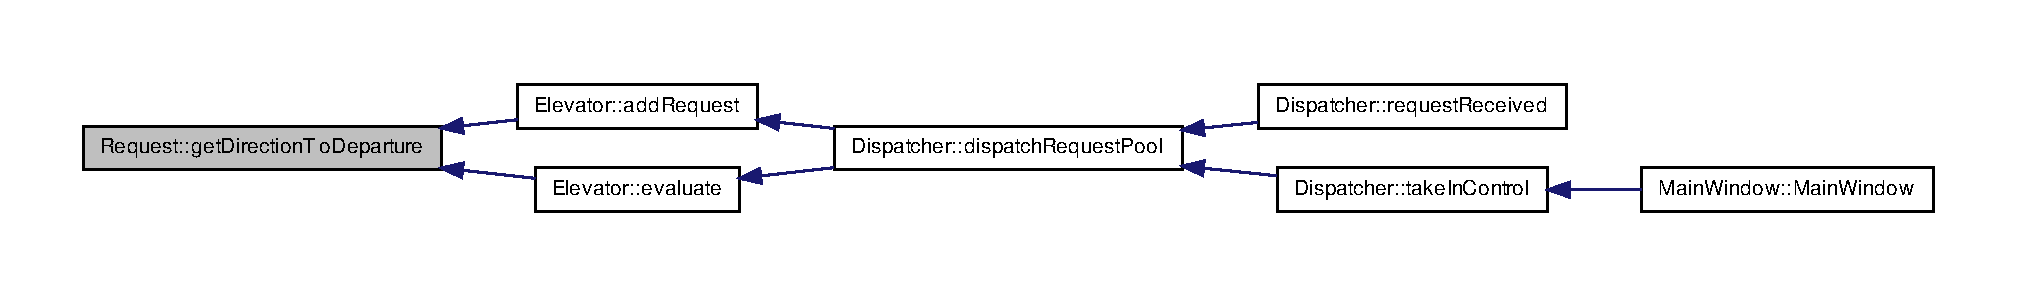
\includegraphics[width=400pt]{class_request_a7a435c886ed19acb556dc2445a53bd37_icgraph}
\end{center}
\end{figure}


\hypertarget{class_request_aeae53642527adaf40498ec5b05921ca0}{
\index{Request@{Request}!getDirectionToDestination@{getDirectionToDestination}}
\index{getDirectionToDestination@{getDirectionToDestination}!Request@{Request}}
\subsubsection[{getDirectionToDestination}]{\setlength{\rightskip}{0pt plus 5cm}{\bf DIRECTION} Request::getDirectionToDestination (
\begin{DoxyParamCaption}
\item[{int}]{floor}
\end{DoxyParamCaption}
)\hspace{0.3cm}{\ttfamily  \mbox{[}inline\mbox{]}}}}
\label{class_request_aeae53642527adaf40498ec5b05921ca0}
Get the the DIRECTION from destination floor to the floor passed. \hypertarget{class_request_a78b24de8cdef27ff340b28d49d251720}{
\index{Request@{Request}!getLength@{getLength}}
\index{getLength@{getLength}!Request@{Request}}
\subsubsection[{getLength}]{\setlength{\rightskip}{0pt plus 5cm}int Request::getLength (
\begin{DoxyParamCaption}
{}
\end{DoxyParamCaption}
)\hspace{0.3cm}{\ttfamily  \mbox{[}inline\mbox{]}}}}
\label{class_request_a78b24de8cdef27ff340b28d49d251720}
Get the the length(floor count) from departure floor to destiination floor. 

Here is the caller graph for this function:\nopagebreak
\begin{figure}[H]
\begin{center}
\leavevmode
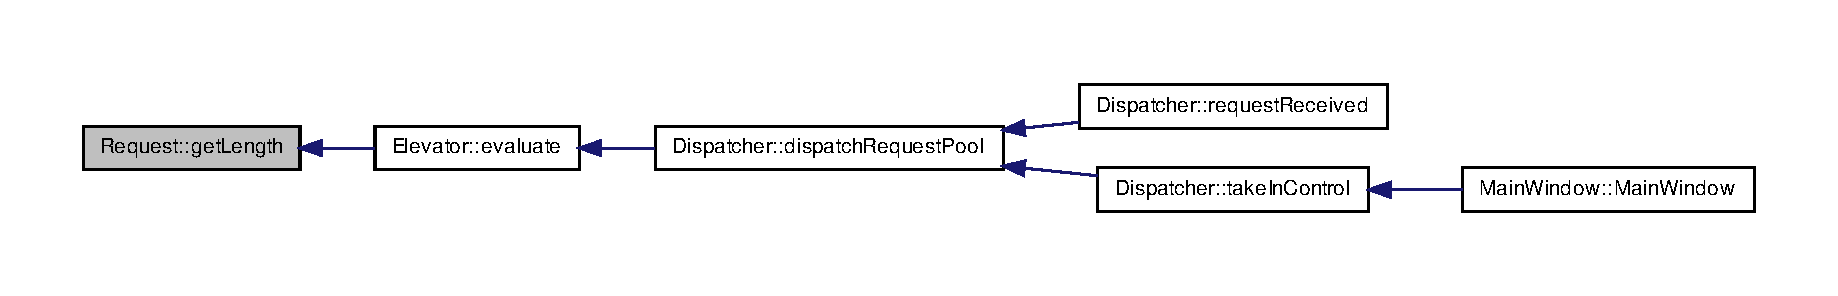
\includegraphics[width=400pt]{class_request_a78b24de8cdef27ff340b28d49d251720_icgraph}
\end{center}
\end{figure}


\hypertarget{class_request_a76a1f5a44df4120828d34a90fbcec13e}{
\index{Request@{Request}!unsetDeparture@{unsetDeparture}}
\index{unsetDeparture@{unsetDeparture}!Request@{Request}}
\subsubsection[{unsetDeparture}]{\setlength{\rightskip}{0pt plus 5cm}void Request::unsetDeparture (
\begin{DoxyParamCaption}
{}
\end{DoxyParamCaption}
)\hspace{0.3cm}{\ttfamily  \mbox{[}inline\mbox{]}}}}
\label{class_request_a76a1f5a44df4120828d34a90fbcec13e}
Mark the departure floor of the \hyperlink{class_request}{Request} to FLOOR\_\-NONE, this usually means that the departure floor of the \hyperlink{class_request}{Request} has been arrived. \hypertarget{class_request_addbd9fdcd5e5a0291c89aad38f6c8416}{
\index{Request@{Request}!unsetDestination@{unsetDestination}}
\index{unsetDestination@{unsetDestination}!Request@{Request}}
\subsubsection[{unsetDestination}]{\setlength{\rightskip}{0pt plus 5cm}void Request::unsetDestination (
\begin{DoxyParamCaption}
{}
\end{DoxyParamCaption}
)\hspace{0.3cm}{\ttfamily  \mbox{[}inline\mbox{]}}}}
\label{class_request_addbd9fdcd5e5a0291c89aad38f6c8416}
Mark the destination floor of the \hyperlink{class_request}{Request} to FLOOR\_\-NONE, define it but seemed that it's useless now. 

\subsection{Member Data Documentation}
\hypertarget{class_request_a9bf9e694beed6b73dd9eaf3f3a73708b}{
\index{Request@{Request}!FLOOR\_\-NONE@{FLOOR\_\-NONE}}
\index{FLOOR\_\-NONE@{FLOOR\_\-NONE}!Request@{Request}}
\subsubsection[{FLOOR\_\-NONE}]{\setlength{\rightskip}{0pt plus 5cm}const int {\bf Request::FLOOR\_\-NONE} = -\/1\hspace{0.3cm}{\ttfamily  \mbox{[}static\mbox{]}}}}
\label{class_request_a9bf9e694beed6b73dd9eaf3f3a73708b}
Value for a floor number hich means unavaliable 

The documentation for this class was generated from the following file:\begin{DoxyCompactItemize}
\item 
request.h\end{DoxyCompactItemize}

\printindex
\end{document}
